\documentclass[12pt]{article}


%\usepackage{showkeys}
%\usepackage{drftcite}
\usepackage{exscale,relsize}
\usepackage{amsmath}
\usepackage{amsfonts}
\usepackage[colorlinks=true, linkcolor=blue]{hyperref}
\usepackage{amssymb}
\usepackage{calc}
\usepackage{theorem}
\usepackage{pifont}      % needed by dingautolist
\usepackage{array}
\usepackage{color}
\usepackage{enumerate}
\usepackage{bbm}
\usepackage{graphicx}
\usepackage{subcaption}
\usepackage{caption}

% \usepackage{amsthm}


% Hongda's packages
\usepackage{algpseudocode, algorithm}
\usepackage{mathtools}


% IF use the below packge, use `\printbibliography' to print out the bibliograph 
% For this one 
% 
% \usepackage[
%     backend=biber,
%     style=numeric,
%     sorting=nyt
% ]{biblatex}
% \addbibresource{references/PPM.bib}
% \addbibresource{references/NesterovMomentum.bib}
% \addbibresource{references/Books.bib}
% \addbibresource{references/BregmanDiv.bib}

% FORMATTING ===================================================================
\oddsidemargin -0.1cm
\textwidth  16.5cm
\topmargin  0.0cm
\headheight 0.0cm
\textheight 21.0cm
\parindent  4mm
\parskip    10pt
%\parskip    8pt
\tolerance  3000

% DRAFT FORMATTING =============================================================
% These are for todo notes, advise taken from 
% https://tex.stackexchange.com/questions/81666/extend-page-width-or-margin-for-todonotes-comments-or-other-package-comments
% \oddsidemargin=\dimexpr\oddsidemargin + 3cm\relax % DON'T USE

\ifthenelse{\boolean{draftmode}}{
    \evensidemargin=\dimexpr\evensidemargin  + 6cm\relax 
    \oddsidemargin=\dimexpr\oddsidemargin + 6cm\relax
    \paperwidth=\dimexpr \paperwidth + 12cm\relax 
    \marginparwidth=\dimexpr \marginparwidth  + 6cm\relax
    \paperheight=\dimexpr \paperheight + 6cm\relax
}{
    
}


% THEOREM AND ENVIRONMENTS.  ===================================================

%\newenvironment{deflist}[1][\quad]%
%{\begin{list}{}{\renewcommand{\makelabel}[1]{\textrm{##1~}\hfil}%
%\settowidth{\labelwidth}{\textrm{#1~}}%
%\setlength{\leftmargin}{\labelwidth+\labelsep}}}%requires macro calc.sty
%{\end{list}}
%\newtheorem{theorem}{Theorem}%[section]
\newtheorem{theorem}{Theorem}[section]
\newtheorem{lemma}[theorem]{Lemma}
\newtheorem{fact}[theorem]{Fact}
\newtheorem{corollary}[theorem]{Corollary}
\newtheorem{proposition}[theorem]{Proposition}
\newtheorem{definition}[theorem]{Definition}
\newtheorem{conjecture}[theorem]{Conjecture}
\newtheorem{observation}[theorem]{Observation}
\newtheorem{openprob}[theorem]{Open Problem}
\theoremstyle{plain}{\theorembodyfont{\rmfamily}
\newtheorem{assumption}[theorem]{Assumption}}
\theoremstyle{plain}{\theorembodyfont{\rmfamily}
\newtheorem{condition}[theorem]{Condition}}
\theoremstyle{plain}{\theorembodyfont{\rmfamily}}

% Removed due conflict with the algorithm environment. 
% \newtheorem{algorithm}[theorem]{Algorithm}}

\theoremstyle{plain}{\theorembodyfont{\rmfamily}
\newtheorem{example}[theorem]{Example}}
\theoremstyle{plain}{\theorembodyfont{\rmfamily}
\newtheorem{remark}[theorem]{Remark}}
\theoremstyle{plain}{\theorembodyfont{\rmfamily}
\newtheorem{application}[theorem]{Application}}

\def\proof{\noindent{\it Proof}. \ignorespaces}
%\def\endproof{\vbox{\hrule height0.6pt\hbox{\vrule height1.3ex%
%width0.6pt\hskip0.8ex\vrule width0.6pt}\hrule height0.6pt}}
%\numberwithin{equation}{section}
\def\endproof{\ensuremath{\quad \hfill \blacksquare}}

\renewcommand\theenumi{(\roman{enumi})}
\renewcommand\theenumii{(\alph{enumii})}
\renewcommand{\labelenumi}{\rm (\roman{enumi})}
\renewcommand{\labelenumii}{\rm (\alph{enumii})}

\numberwithin{equation}{section}



% These are Heniz's notations. 
\newcommand{\To}{\ensuremath{\rightrightarrows}}
\newcommand{\GX}{\ensuremath{\Gamma}}
\newcommand{\mal}{\ensuremath{\mathfrak{m}}}
\newcommand{\mumu}{\ensuremath{{\mu\mu}}}
\newcommand{\paver}{\ensuremath{\mathcal{P}}}
\newcommand{\ZZZ}{\ensuremath{{X \times X^*}}}
\newcommand{\RRR}{\ensuremath{{\RR \times \RR}}}
\newcommand{\todo}{\hookrightarrow\textsf{TO DO:}}

\newcommand{\emp}{\ensuremath{\varnothing}}
%\newcommand{\la}{\ensuremath{\langle}}
%\newcommand{\ra}{\ensuremath{\rangle}}
\newcommand{\infconv}{\ensuremath{\mbox{\small$\,\square\,$}}}
\newcommand{\pscal}{\ensuremath{\scal{\cdot}{\cdot}}}
\newcommand{\Tt}{\ensuremath{\mathfrak{T}}}
\newcommand{\YY}{\ensuremath{\mathcal Y}}
\newcommand{\XX}{\ensuremath{\mathcal X}}
\newcommand{\HH}{\ensuremath{\mathcal H}}
\newcommand{\XP}{\ensuremath{\mathcal X}^*}
\newcommand{\st}{\ensuremath{\;|\;}}
\newcommand{\zeroun}{\ensuremath{\left]0,1\right[}}

\newcommand{\lev}[1]{\ensuremath{\mathrm{lev}_{\leq #1}\:}}
\newcommand{\moyo}[2]{\ensuremath{\sideset{_{#2}}{}{\operatorname{}}\!#1}}
\newcommand{\pair}[2]{\left\langle{{#1},{#2}}\right\rangle}
%\newcommand{\scal}[2]{\left.\left\langle{#1}\:\right| {#2}  \right\rangle}
\newcommand{\scal}[2]{\langle{{#1},{#2}}\rangle}
\newcommand{\Scal}[2]{\left\langle{{#1},{#2}}\right\rangle}
%\newcommand{\scal}[2]{\braket{ {#1},{#2}}}

\newcommand{\yosida}{\ensuremath{ \; {}^}}
\newcommand{\exi}{\ensuremath{\exists\,}}
\newcommand{\GG}{\ensuremath{\mathcal G}}
\newcommand{\RR}{\ensuremath{\mathbb R}}
\newcommand{\SSS}{\ensuremath{\mathbb S}}
\newcommand{\CC}{\ensuremath{\mathbb C}}
\newcommand{\Real}{\ensuremath{\mathrm{Re}\,}}
\newcommand{\ii}{\ensuremath{\mathrm i}}
\newcommand{\RP}{\ensuremath{\left[0,+\infty\right[}}
\newcommand{\RPX}{\ensuremath{\left[0,+\infty\right]}}
\newcommand{\RPP}{\ensuremath{\,\left]0,+\infty\right[}}
\newcommand{\RX}{\ensuremath{\,\left]-\infty,+\infty\right]}}
\newcommand{\RXX}{\ensuremath{\,\left[-\infty,+\infty\right]}}
\newcommand{\KK}{\ensuremath{\mathbb K}}
\newcommand{\NN}{\ensuremath{\mathbb N}}
\newcommand{\nnn}{\ensuremath{{n \in \NN}}}
\newcommand{\thalb}{\ensuremath{\tfrac{1}{2}}}
\newcommand{\zo}{\ensuremath{{\left]0,1\right]}}}
\newcommand{\lzo}{\ensuremath{{\lambda \in \left]0,1\right]}}}
%\newcommand{\toppsepp}{\setlength{\partopsep}{-5pt}}
\newcommand{\menge}[2]{\big\{{#1} \mid {#2}\big\}}
\newcommand{\pfrac}[2]{\ensuremath{\mathlarger{\tfrac{#1}{#2}}}}


% MATH OPERATORS ===============================================================
% \newcommand{\monos}{\ensuremath{\mathcal M}}
\newcommand{\DD}{\operatorname{dom}f}
\newcommand{\IDD}{\ensuremath{\operatorname{int}\operatorname{dom}f}}
\newcommand{\CDD}{\ensuremath{\overline{\operatorname{dom}}\,f}}
\newcommand{\clspan}{\ensuremath{\overline{\operatorname{span}}}}
\newcommand{\cone}{\ensuremath{\operatorname{cone}}}
\newcommand{\dom}{\ensuremath{\operatorname{dom}}}
\newcommand{\closu}{\ensuremath{\operatorname{cl}}}
\newcommand{\cont}{\ensuremath{\operatorname{cont}}}
\newcommand{\mons}{\ensuremath{\mathcal{A}}}
\newcommand{\gra}{\ensuremath{\operatorname{gra}}}
\newcommand{\epi}{\ensuremath{\operatorname{epi}}}
\newcommand{\prox}{\ensuremath{\operatorname{Prox}_{\mu}}}
\newcommand{\hprox}{\ensuremath{\operatorname{prox}}}
\newcommand{\intdom}{\ensuremath{\operatorname{int}\operatorname{dom}}\,}
\newcommand{\inte}{\ensuremath{\operatorname{int}}}
\newcommand{\sri}{\ensuremath{\operatorname{sri}}}
\newcommand{\reli}{\ensuremath{\operatorname{ri}}}
\newcommand{\cart}{\ensuremath{\mbox{\LARGE{$\times$}}}}


\newcommand{\average}{\ensuremath{\mathcal{R}_{\mu}({\bf A},{\boldsymbol \lambda})}}
\newcommand{\averagebar}{\ensuremath{\mathcal{R}_{1}({\bf A},\bar{\lambda})}}
\newcommand{\averageonelambda}{\ensuremath{\mathcal{R}({\bf A},{\boldsymbol \lambda})}}
\newcommand{\averageonehalf}{\ensuremath{\mathcal{R}_{1}(A,1/2)}}
\newcommand{\averageinverse}{\ensuremath{\mathcal{R}_{\mu^{-1}}({\bf A}^{-1},{\boldsymbol \lambda})}}
\newcommand{\averageoneinverse}{\ensuremath{\mathcal{R}({\bf A}^{-1},{\boldsymbol \lambda})}}
\newcommand{\averagef}{\ensuremath{\mathcal{P}_{\mu}(f,\lambda)}}
\newcommand{\averagefone}{\ensuremath{\mathcal{P}_{1}(f,\lambda)}}
\newcommand{\averagefd}{\ensuremath{\mathcal{P}_{\mu}((f_{1},\ldots, f_{n}),(\lambda_{1},\ldots, \lambda_{n}))}}
\newcommand{\averagefik}{\ensuremath{\mathcal{P}_{\mu_{k}}((f_{1,k},\ldots,f_{n,k}),
(\lambda_{1,k},\ldots,\lambda_{n,k}))}}
\newcommand{\averagesub}{\ensuremath{\mathcal{R}_{\mu}(\partial f,\lambda)}}
\newcommand{\res}{\ensuremath{\mathcal{R}_{\mu}}}
\newcommand{\resmuk}{\ensuremath{\mathcal{R}_{\mu_{k}}}}
\newcommand{\newres}{\ensuremath{\mathcal{R}}}
\newcommand{\resmualpha}{\ensuremath{\mathcal{R}_{\alpha\mu}}}
\newcommand{\averageone}{\ensuremath{\mathcal{R}_{1}}}
\newcommand{\harm}{\ensuremath{\mathcal{H}(A,\lambda)}}
\newcommand{\arithmetic}{\ensuremath{\mathcal{A}(A,\lambda)}}

\newcommand{\WC}{\ensuremath{{\mathfrak W}}}
\newcommand{\SC}{\ensuremath{{\mathfrak S}}}
\newcommand{\card}{\ensuremath{\operatorname{card}}}
\newcommand{\bd}{\ensuremath{\operatorname{bdry}}}
\newcommand{\ran}{\ensuremath{\operatorname{ran}}}
\newcommand{\rec}{\ensuremath{\operatorname{rec}}}
\newcommand{\rank}{\ensuremath{\operatorname{rank}}}
\newcommand{\kernel}{\ensuremath{\operatorname{ker}}}
\newcommand{\conv}{\ensuremath{\operatorname{conv}}}
\newcommand{\segh}{\ensuremath{\operatorname{seg}}}
\newcommand{\boxx}{\ensuremath{\operatorname{box}}}
\newcommand{\clconv}{\ensuremath{\overline{\operatorname{conv}}\,}}
\newcommand{\cldom}{\ensuremath{\overline{\operatorname{dom}}\,}}
\newcommand{\clran}{\ensuremath{\overline{\operatorname{ran}}\,}}
\newcommand{\Nf}{\ensuremath{\nabla f}}
\newcommand{\NNf}{\ensuremath{\nabla^2f}}
\newcommand{\Fix}{\ensuremath{\operatorname{Fix}}}
\newcommand{\FFix}{\ensuremath{\overline{\operatorname{Fix}}\,}}
\newcommand{\aFix}{\ensuremath{\widetilde{\operatorname{Fix}\,}}}
\newcommand{\Id}{\ensuremath{\operatorname{Id}}}
\newcommand{\Max}{\ensuremath{\operatorname{max}}}
\newcommand{\Bb}{\ensuremath{\mathfrak{B}}}
\newcommand{\BB}{\ensuremath{\mathbb{B}}}
\newcommand{\Fb}{\ensuremath{\overrightarrow{\mathfrak{B}}}}
\newcommand{\Fprox}{\ensuremath{\overrightarrow{\operatorname{prox}}}}
\newcommand{\Bprox}{\ensuremath{\overleftarrow{\operatorname{prox}}}}
\newcommand{\Bproj}{\ensuremath{\overleftarrow{\operatorname{P}}}}
\newcommand{\Ri}{\ensuremath{\mathfrak{R}_i}}
\newcommand{\Dn}{\ensuremath{\,\overset{D}{\rightarrow}\,}}
\newcommand{\nDn}{\ensuremath{\,\overset{D}{\not\rightarrow}\,}}
\newcommand{\weakly}{\ensuremath{\,\rightharpoonup}\,}
\newcommand{\weaklys}{\ensuremath{\,\overset{*}{\rightharpoonup}}\,}
\newcommand{\gr}{\ensuremath{\operatorname{gra}}}
\newcommand{\g}{\ensuremath{\,\overset{g}{\rightarrow}}\,}
\newcommand{\p}{\ensuremath{\,\overset{p}{\rightarrow}}\,}
\newcommand{\e}{\ensuremath{\,\overset{e}{\rightarrow}}\,}
\newcommand{\Tbar}{\ensuremath{\overline{T}}}
\newcommand{\n}{\ensuremath{\,\overset{n}{\rightarrow}}\,}

\newcommand{\minf}{\ensuremath{-\infty}}
\newcommand{\pinf}{\ensuremath{+\infty}}
\renewcommand{\iff}{\ensuremath{\Leftrightarrow}}
% \renewcommand{\phi}{\ensuremath{\varphi}}
%\newcommand{\Real}{\ensuremath{\mathrm{Re}\,}}
\newcommand{\negent}{\ensuremath{\operatorname{negent}}}
\newcommand{\neglog}{\ensuremath{\operatorname{neglog}}}
\newcommand{\halb}{\ensuremath{\tfrac{1}{2}}}
\newcommand{\bT}{\ensuremath{\mathbf{T}}}
\newcommand{\bX}{\ensuremath{\mathbf{X}}}
\newcommand{\bL}{\ensuremath{\mathbf{L}}}
\newcommand{\bD}{\ensuremath{\boldsymbol{\Delta}}}
\newcommand{\bc}{\ensuremath{\mathbf{c}}}
\newcommand{\by}{\ensuremath{\mathbf{y}}}
\newcommand{\bx}{\ensuremath{\mathbf{x}}}
\newcommand{\bA}{{\bf A}}
\newcommand{\Other}{Indeterminate }
\newcommand{\other}{indeterminate }


%%% Raf's stuff  ===============================================================
\newcommand{\al}{\alpha}
\newcommand{\la}{\lambda}
\newcommand{\La}{\Lambda}
\newcommand{\pluss}{{\hskip1pt \raise1pt\vbox{\hrule width6pt \vskip1pt
\hrule width6pt}\kern-4pt{\lower1pt\hbox{\vrule height6pt \kern1pt\vrule
height6pt}}\hskip5pt}}
\newcommand{\timess}{\star}
\newcommand{\argmax}{\mathop{\rm argmax}\limits}
\newcommand{\argmin}{\mathop{\rm argmin}\limits}
\newcommand{\product}{\langle\cdot,\cdot\rangle}
\newcommand{\im}{\mathrm{Im}}
\newcommand{\multival}{\ensuremath{X\to 2^{X^*}}}
\newcommand{\SX}{\ensuremath{2^{X^*}}}

\newcommand{\inlinecode}[1]{\texttt{\footnotesize #1}}

\usepackage{listings} \lstset{basicstyle=\footnotesize\ttfamily,breaklines=true}
\usepackage{xcolor}
\lstdefinelanguage{Julia}%
  {morekeywords={abstract,break,case,catch,const,continue,do, else, elseif,%
      end, export, false, for, function, immutable, import, importall, if, in,%
      macro, module, otherwise, quote, return, switch, true, try, type, typealias,%
      using, while},%
   sensitive=true,%
   alsoother={$},%
   morecomment=[l]\#,%
   morecomment=[n]{\#=}{=\#},%
   morestring=[s]{"}{"},%
   morestring=[m]{'}{'},%
}[keywords,comments,strings]%
\lstset{%
    language         = Julia,
    basicstyle       = \ttfamily,
    keywordstyle     = \bfseries\color{blue},
    stringstyle      = \color{magenta},
    commentstyle     = \color{ForestGreen},
    showstringspaces = false,
}

% === TEMPLATE HOW TO USE ======
% To begine here is a list of things: 
% [ ]: Change title. 
% [ ]: Fill into the author names, affiliation and contact info. 
% [ ]: Fill in the abstract. 
% [ ]: Fill/change in AMS mathematics subject classification code, and the keywords. 

\title{
    {
        \fontfamily{ptm}\selectfont 
        First Order Nonsmooth Optimization: 
        Algorithm Design, Variational analysis, and Applications
    }
}
\author{
    % \thanks{Department of Mathematics, I.K. Barber Faculty of Science,
    % The University of British Columbia, Kelowna, BC Canada V1V 1V7. 
    % E-mail:  \texttt{alto@mail.ubc.ca}.}~Hongda Li
    % \thanks{Department of Mathematics, I.K. Barber Faculty of Science,
    % The University of British Columbia, Kelowna, BC Canada V1V 1V7. 
    % E-mail:  \texttt{shawn.wang@ubc.ca}.}~ and~Author Name 2
    Hongda Li\\[3ex]\\ Department of Mathematics\\
	University of British Columbia,\\
	Okanagan Campus.
}
\date{\today}

\begin{document}
% \vspace{10ex}
% \vskip 8mm

\maketitle
\tableofcontents
\pagebreak



% \begin{abstract} 
%     \noindent
%     The research proposal focuses on the theories and practice in solving nonsmooth optimization. 
%     The theme of proposal highlight topics of interests that emphasize the computations and applications aspect of algorithms that exhibits both practical and theoretical importance. 
%     We summarize our ongoing research in unifying Nesterov type accelerated proximal gradient method and proposes our Free R-WAPG method. 
%     We survey literatures under the topic of Catalyst Meta Acceleration framework used in accelerating variance reduced methods in the settings of Data Science and Machine Learning. 
%     Furthermore, we present literatures and progress in topics such as Performance Estimation Problem, Inexact Proximal Point, acceleration without convexity. 
%     At the end there is a section summarizing a method we developed for tree species classifications using Sentinel-2 satellite remote sensing data using big data analytics by extract spectral signatures of ground vegetation covers. 


% \end{abstract}
% \noindent{\bfseries 2010 Mathematics Subject Classification:}
% Primary 65K10, 90c25, 90C30; Secondary 65Y20. 
% \noindent{\bfseries Keywords: } Non-convex Optimizations, Proximal Point. 


\section{Introduction}
    Let $\RR^n$ be the ambient space. We consider 
    \begin{align}
        \min_{x \in \RR^n} \left\lbrace
            F(x): f(x) + g(x)
        \right\rbrace.
    \end{align}\label{eqn:additive-comp-obj}
    Unless specified, assume $f:\RR^n \rightarrow \RR$ is $L$-Lipscthiz smooth $\mu \ge 0$ strongly convex and $g:Q \rightarrow \overline \RR$ is convex. 
    This type of problem is referred to as additive composite problems in the literature. 
    \par
    Our ongoing research concerns accelerated proximal gradient type method for solving (\ref{eqn:additive-comp-obj}). 
    In the expository writing by Walkington \cite{noel_nesterovs_nodate}, a variant for of accelerated gradient method for strongly convex function $f$ is discussed. 
    We had two lingering questions after reading it. 
    \begin{enumerate}
        \item Do there exist a unified description for the convergence for both variants of the algorithms?
        \item Is it possible to attain faster convergence rate without knowledge about the strong convexity of function $f$?
        \item Is it possible to describe the convergence of function value for momentum sequences that are much weaker than the Nesterov's rule? 
    \end{enumerate}
    The good news is we have definitive answers for all questions by our own efforts of research. 
    Section \ref{sec:unify-nes-acceleration}, \ref{sec:spectral-momentum} are our ongoing research which present the answers to the questions. 
    \par
    In Section \ref{sec:unify-nes-acceleration}, we proposed the method of ``Relaxed Weak Accelerated Proximal Gradient (R-WAPG)'' as the foundation to describe several variants of Accelerated proximal gradient method in the literatures. 
    The convergence theories of R-WAPG allows us to model convergence of accelerated proximal gradient method where the momentum sequence doesn't strictly follow the conditions presented in the literatures. 
    The descriptive power of R-WAPG allows convergence analysis for all the variants using one single theorem. 
    \par
    In Section \ref{sec:spectral-momentum} we propose a practical algorithm that exploits a specific term in the proof of R-WAPG to achieve faster convergence for solving (\ref{eqn:additive-comp-obj}) without knowing parameter $L, \mu$ in prior. 
    Results of numerical experiments are presented. 
    \par
    Section \ref{sec:catalyst} are results of literatures review in MATH 590. 
    \todo{
        $\blacksquare$ Add Lin's papers and Paquette's papers.
    }
    {\hl{It's based on a series of papers}} in the topic of Catalyst Meta Acceleration method for First Order Variance Reduced Methods. 
    We will point out potential future direction of research of Catalyst acceleration. 
    \par
    Section \ref{sec:inexact-prox}, \ref{sec:nes-acc-ncnvx} preview literatures in nonsmooth optimization frontier research where progress and impacts can be made.  
    \subsection{Theme of the research}
        This section specifies a theme of the research in this proposal. 
        Out first objective is to explore the Goldilocks zones between these topics: theories of variational analysis, design of continuous optimization algorithm and applications in sciences, engineering, and statistics.  
        Our second objective is to identify the ``chemistry'' occurring between properties of functions and the designs of continuous optimizations algorithm and how it impacts the convergence and behaviors of the algorithms. 


    
\section{Preliminaries}
    \todoinline{
        Clarify: Notations,
        Organizations. 
    }
    This section contains the basics of contents from convex optimization, and variational analysis. 
    \par
    Notations. 
    \begin{enumerate}
        \item $\overline \RR := \RR \cup \{\infty, -\infty\}$
    \end{enumerate}
    \subsection{Fundamentals in non-convex analysis}
        Let the ambient space be $\RR^n$ equipped with inner product and 2-norm. 
        Let $O$ be an open subset of $\RR^n$, the weakest assumption we are making for the objective function $F: O \subseteq \RR^n \rightarrow \RR$ for optimization problem is Local Lipschitz Continuity. 
        The assumption of local Lipschitz continuity is weak enough to describe most problems in applications, and strong enough to avoid most pathologies in analysis. 

        \begin{definition}[Local Lipschitz continuity]
            Let $F: O \subseteq \RR^n \rightarrow \RR$ be Locally Lipschitz and $O$ is an open set. 
            Then for all $\bar x \in O$, there exists a Neighborhood: $\mathcal N(\bar x)$ and $K \in \RR$ such that for all $x, y \in \mathcal N(\bar x)$: $|F(x) - F(y)| \le K \Vert x - y\Vert$. 
        \end{definition}
        \begin{definition}[Regular subgradient]
            Let $F: O \subseteq \RR^n \rightarrow \RR$ be locally Lipschitz and $\bar x \in O$. 
            The regular subdifferential at $\bar x$ is defined as 
            \begin{align*}
                \widehat \partial F(\bar x) := 
                \left\lbrace
                    v \in \RR^n \left| \; 
                        \liminf_{\bar x \neq x\rightarrow \bar x}
                        \frac{F(x) - F(\bar x) - \langle v, x - \bar x\rangle}{\Vert x - \bar x\Vert} 
                        \ge 0
                    \right.
                \right\rbrace. 
            \end{align*}
        \end{definition}
        \begin{remark}
            Definition taken from Definition 4.3.1 from 
            \todo{$\blacksquare$ Add bib \\ $\blacksquare$ Cite. }
            \hl{Pang, Cui's book} \cite{ying_modern_2021}
        \end{remark}
        \begin{definition}[Limiting subgradient]
            Let $F: O \subseteq \RR^n \rightarrow \RR$ be locally Lipschitz and $\bar x \in O$. 
            The limiting subdifferential at $\bar x$ is defined as 
            \begin{align*}
                \partial F(\bar x) := 
                \left\lbrace
                    v \in \RR^n \left| \; 
                        \exists x_k \rightarrow \bar x, v_k \rightarrow v: 
                        v_k \in \widehat \partial F(x_k) \;\forall k \in \mathbb N
                    \right.
                \right\rbrace. 
            \end{align*}
        \end{definition}
        \begin{remark}
            Definition taken from Definition 4.3.1 from
            \todo{$\blacksquare$ Add bib \\ $\blacksquare$ Cite. }
            {\hl{Pang, Cui's book}} \cite{ying_modern_2021}
        \end{remark}
        \begin{definition}[Weakly convex function]
            $F: \RR^n \rightarrow \overline \RR$ is $\mu$ weakly convex if and only if $F + \frac{\mu}{2}\Vert \cdot\Vert^2$ is convex. 
        \end{definition}
        \begin{definition}[Bregman divergence]
            Let $F: O \subseteq \RR^n \rightarrow \RR$ be a differentiable function. 
            Then the Bregman divergence of $F$ is defined as: 
            \begin{align*}
                D_F(x, y): O \times \dom(\partial F) \rightarrow \RR
                := F(x) - F(y) - \langle \nabla F(y), x - y\rangle. 
            \end{align*}
        \end{definition}
    \subsection{Fundamentals in convex analysis}
        This section introduces the classics and basics of convex analysis. 
        Define $F$ to be closed, proper and convex in this section. 
        When $F$ is convex, the limiting subgradient and the regular subgradient reduced to the following definition:
        \begin{align*}
            \partial F(x) := \left\lbrace
                v \in \RR^n \left|\; 
                    \forall y \in \RR^n\; :  F(y) - F(x)  \ge \langle v, y - x\rangle
                \right.
            \right\rbrace. 
        \end{align*}
        A convex function is locally Lipschitz in the relative interior of its domain, denoted as $\reli(\dom(F))$. 
        So it has $\reli(\dom F)\subseteq \dom(\partial F) \subseteq \dom F$. 
        \par
        When we say $F:\RR^n \rightarrow \RR$ is $L$ Lipschitz smooth function, it means that there exists $L$ such that for all $x\in \RR^n, y \in \RR^n$, it has: 
        \begin{align*}
            \Vert \nabla F(x) - \nabla F(y)\Vert \le L \Vert x - y\Vert. 
        \end{align*}
        This condition is stronger than differentiability. 
        When $F$ convex, it has descent lemma: 
        \begin{align*}
            (\forall x \in \RR^n)(\forall y \in \RR^n): 0 \le 
            F(x) - F(y) - \langle \nabla f(y), x - y\rangle \le \frac{L}{2}\Vert x - y\Vert^2. 
        \end{align*}
        When $F$ is convex, the converse holds. 
        The definitions that follow narrow things further for future discussions. 
        \begin{definition}[Strong convexity]\label{def:s-cnvx}
            A function $F:\RR^n \rightarrow \overline \RR$ is $\mu \ge 0$ strongly convex if and only if for any fixed $y \in \dom(\partial F)$, we have for all $x\in \RR^n$: 
            \begin{align*}
                (\forall v \in \partial F(x))\quad 
                F(x) - F(y) \ge \langle v, x - y\rangle + \frac{\mu}{2}\Vert x - y\Vert^2. 
            \end{align*}
        \end{definition}
        \begin{lemma}[Quadratic growth from strong convexity]\label{lemma:q-growth}
            If $F$ is $\mu \ge 0$ strongly convex, $\bar x$ is a minimizer of $F$. 
            Then for all $x \in \RR^n$
            \begin{align*}
                F(x) - F(\bar x) \ge \frac{\mu}{2}\Vert x - \bar x\Vert^2. 
            \end{align*}
        \end{lemma}
        \begin{remark}
            The minimizer is unique whenever $\mu > 0$. 
            For contradiction, assume $x$ is another minimizer, then $F(x) \neq F(\bar x)$, which is a direct contradiction. 
            The quadratic growth condition over a set of minimizer is much weaker than convexity. 
        \end{remark}
        
        \subsubsection{Smooth, nonsmooth additive composite}\label{sssec:additive-composite}
            In this section, we zoom in further. 
            Suppose that $F:= f + g$ where $f:\RR^n \rightarrow \RR$ is convex, $L$ Lipschitz smooth and $\mu \ge 0$ strongly convex and $g: \RR\rightarrow \overline \RR$ is convex. 
            To make the discussion simpler, fix any $\beta \ge 0$ we define the following model functions as a $\RR^n \times \RR^n \rightarrow \overline \RR$: 
            \begin{align*}
                \widetilde{\mathcal M}^{\beta^{-1}}
                (x; y)
                &:= 
                g(x) + f(y) + \langle \nabla f(y), x - y\rangle
                + \frac{\beta}{2}\Vert x - y\Vert^2,
                \\
                \mathcal M^{\beta^{-1}}(x; y) 
                &:= F(x) + \frac{\beta}{2}\Vert x - y\Vert^2.
            \end{align*}
            Under convexity assumption in this section, both $\widetilde {\mathcal M} (\cdot; y),  {\mathcal M}(\cdot;y )$ is at least $\beta \ge 0$ strongly convex. 
            \begin{definition}[Proximal gradient operator]\label{def:proximal-gradient-operator}
                Take $F := f + g$ where $g: \RR^n \rightarrow \overline \RR$ as defined in this section. 
                Define the proximal gradient operator $T_L$ on all $y \in \RR^n$: 
                \begin{align*}
                    T_L y := \argmin_{x \in \RR^n} \left\lbrace
                        g(x) + f(y) + \langle \nabla f(y), x - y\rangle 
                        + \frac{L}{2}\Vert x- y \Vert^2
                    \right\rbrace. 
                \end{align*}
            \end{definition}
            \begin{remark}
                Under the assumption of this section, the mapping $T_L$ is a single-valued mapping, it has domain on the entire $\RR^n$, and it's a $3/2$ averaged operator. 
            \end{remark}
            \begin{definition}[Gradient mapping operator]\label{def:gradient-mapping-operator}
                Take $F := f + g$ as defined in this section. 
                Define the gradient mapping operator $\mathcal G_L$ on all $y \in \RR^n$: 
                \begin{align*}
                    \mathcal G_L y:= L(y - T_L y). 
                \end{align*}
            \end{definition}

            \begin{lemma}[Proximal gradient model function]\;\\
                Take $\widetilde{\mathcal M}^{L^{-1}}, \mathcal M^{L^{-1}}$ as defined in this section, we will have for all $x \in \RR^n$ that: 
                \begin{align*}
                    \widetilde{\mathcal M}^{L^{-1}}(x; y)
                    &= 
                    \mathcal M^{L^{-1}}(x; y)- D_f(x, y).
                \end{align*}
            \end{lemma}
            \begin{lemma}[A favorable property of gradient mapping]
                Take $F:= f + g$ as defined in this section. 
                Fix any $x \in \RR^n$. 
                Then there exists $v \in \partial g(T_L x)$ such that $\mathcal G_L (x) = v + \nabla f(x)$. 
            \end{lemma}
            \begin{remark}
                This lemma still holds for non-convex $f$ under prox-boundedness and weak convexity and differentiability of $f$. 
            \end{remark}
            \begin{lemma}[The proximal gradient inequality]\label{thm:prox-grad-ineq}
                Take $F:= f + g$ as defined in this section. 
                Fix any $y \in \RR^n$, then for all $x$, the proximal gradient inequality is true: 
                \begin{align*}
                    (\forall x \in \RR^n)\quad 
                    h(x)  - h(Ty) - \langle L(y - Ty), x - y\rangle
                    - \frac{\mu}{2}\Vert x - y\Vert^2 - \frac{L}{2}\Vert y - Ty\Vert^2 
                    &\ge 0. 
                \end{align*}
            \end{lemma}
            \begin{remark}
                This lemma is proved in our draft paper. 
            \end{remark}

    \subsection{Nesterov's estimating sequence technique}
        \todoinline{\noindent
            Do the following: 
            \begin{enumerate}
                \item What is Nesterov's estimating sequence. 
                \item How is it used to derive the algorithm and convergence rate of algorithm. 
                \item Where is it used and why is it important here. 
            \end{enumerate}
        }
        \todoinline{
            Examples
            \begin{enumerate}
                \item Example estimating sequence. 
            \end{enumerate}
        }
        The method of Nesterov's estimating sequence for accelerated gradient method, and their nonsmooth counterparts assumes a convex function $F: \RR^n \rightarrow \overline{\RR}$. 
        The estimating sequence is a technique searching for candidate algorithm with extrapolated momentum, and proving their convergence rate if possible. 
        \par
        The method is widespread in the literatures, and the ideas behind it are tremendously useful. 
        \todo{
            $\blacksquare$ Add Guler's 1992 new proximal point paper. 
            \\ $\blacksquare$ Cite it.}
        {\hl{Güler}} \cite{guler_new_1992}
        used the method to design an accelerated proximal point method, which inspired and served as the foundation of Catalyst Acceleration for variance reduced method in machine learning. 
        \todo{
            $\blacksquare$ Add the paper: ``Accelerating the cubic regularization of Newton’s method on convex
            problems''\\ 
            $\blacksquare$ Cite it.
        }
        {\hl{Nesterov}} \cite{nesterov_accelerating_2008}
        also used the technique to design an accelerated cubic regularized Newton's method. 
        In 
        \todo{
            $\blacksquare$ Cite it. 
        }
        \hl{(6.1.19) of Nesterov's book }\cite{nesterov_lectures_2018}, 
        it's also used to derive a method of accelerated mirror descent. 
        And finally, 
        \todo{
            $\blacksquare$ Add paper: ``Accelerated regularized newton methods for minimizing composite convex functions'' \\ 
            $\blacksquare$ Cite it. 
        }
        {\hl{Geovani N. et al}} \cite{grapiglia_accelerated_2019}
        used the technique to derive an accelerated Newton's method for convex composite objective function. 
        \par
        The definition of the estimating sequence that follows is based on our own understanding of the estimating sequence. 
        \begin{definition}[Nesterov's estimating sequence]\label{def:nes-est-seq}
            Let $\phi_k : \RR^n \rightarrow\RR$ for all $k \ge 0$ be a sequence of functions. 
            We call this sequence of function a Nesterov's estimating sequence when it satisfies the conditions: 
            \begin{enumerate}
                \item There exists another sequence $(x_k)_{k \ge 0}$ such that for all $k \ge 0$ it has $F(x_k) \le \phi_k^*: =\min_{x}\phi_k(x)$. 
                \item There exists a sequence of $(\alpha_k)_{k \ge 0}$ where $\alpha_k \in (0, 1)\; \forall k \ge0 $ such that for all $x \in \RR^n$ it has $\phi_{k + 1}(x) - \phi_k(x) \le - \alpha_k(\phi_k(x) - F(x))$. 
            \end{enumerate}
        \end{definition}
        \begin{observation}
            In general, identifying the sequence $(x_k)_{k \ge 0}$ is non-trivial. 
            But in case it can be found, the method of estimating sequence gives us the convergence rate described by the sequence $(\alpha_k)_{k \ge 0}$, and a candidate algorithm that generates the sequence $(x_k)_{k \ge 0}$. 
            It's two birds with one stone. 
            \par 
            If we define $\phi_k$, $\Delta_k(x) := \phi_k (x) - F(x)$ for all $x \in \RR^n$ and assume that $F$ has minimizer $x^*$. 
            Then observe that $\forall k \ge 0$:  
            \begin{align*}
                \Delta_k(x) 
                &= \phi_k(x) - F(x) \ge \phi_k^* - F(x)
                \\
                x = x_k\implies 
                \Delta_k(x_k) 
                &\ge 
                \phi_k^* - F(x_k) \ge 0;
                \\
                x = x_* \implies 
                \Delta_k(x_*)
                &\ge \phi_k^* - F_* \ge F(x_k) - F_* \ge 0. 
            \end{align*}
            The function $\Delta_k(x)$ is non-negative at points: $x_*, x_k$.
            We can derive the convergence rate of $\Delta_k(x^*)$ because $\forall x \in \RR^n$: 
            \begin{align*}
                \phi_{k + 1}(x) - \phi_k(x) 
                &\le - \alpha_k (\phi_k(x) - F(x))
                \\
                \iff 
                \phi_{k + 1}(x) - F(x) - (\phi_k(x) - F(x))
                &\le 
                -\alpha_k(\phi_k(x) - F(x))
                \\
                \iff
                \Delta_{k + 1}(x) - \Delta_k(x) &\le
                - \alpha_k\Delta_k(x)
                \\
                \iff 
                \Delta_{k + 1}(x) 
                &\le 
                (1 - \alpha_k)\Delta_k(x). 
            \end{align*}
            Unrolling the above recursion it yields: 
            \begin{align*}
                \Delta_{k + 1}(x) &\le 
                (1 - \alpha_k)\Delta_k(x) \le \cdots \le 
                \left(
                    \prod_{i = 0}^k(1 - \alpha_i)
                \right)\Delta_0(x). 
            \end{align*}
            Finally, by setting $x = x^*$, $\Delta_k(x^*)$ is non-negative and using the property of Nesterov's estimating sequence it gives: 
            \begin{align*}
                F(x_k) - F(x^*) \le \phi_k^* - F(x^*) \le \Delta_k(x^*) = \phi_k(x^*) - F(x^*) \le \left(\prod_{i = 0}^k(1 - \alpha_i)\right)\Delta_0(x^*).
            \end{align*} 

        \end{observation}
        

\section{Unifying NAG, and weakening the sequence assumption for convergences}\label{sec:unify-nes-acceleration}
    \todoinline{\noindent
        This section is really about stating the results of the draft paper and no proofs will be done here. 
        Along with the content of the draft paper, we will also explain the origin and inspirations of the ideas. 
    }
    This section is based on the theoretical aspects of our draft paper. 
    It will introduce major results and claims achieved during our research in each of the subsections. 
    All theorems and claims stated in this section have proofs in the draft paper. 
    The proofs haven't been carefully verified by authoritative people other than the author yet. 
    We will start introducing the context and ideas for our research next. 
    \par
    Assume we want to solve a convex optimization problem: $\min_{x \in \RR^n} \{F(x)\}$ and $F: \RR^n \rightarrow \RR$ is a $L$ Lipschitz smooth function. 
    We made this assumption for now for a faster exposition. 
    One of the prime candidate for solving the optimization problem is the Nesterov's Accelerated Gradient methods (NAG) finds extensions for nonsmooth function through the proximal gradient operator.
    \todo{
        $\blacksquare$ Add Nesterov's original paper. \\ 
        $\blacksquare$ Cite it.  
    }
    {\hl{Proposed back in 1983 the original Nesterov's acceleration method}} \cite{nesterov_method_1983}
    which uses the previous iterates to extrapolate the next iterate to evaluate the gradient. 
    It's well known that if minimizer $x^*$ exists for $F$, the method achieves a $\mathcal O(1/k^2)$ convergence rate on the objective value $F(x_k)$. 
    \todo{
        $\blacksquare$ Add Nesterov's new book. 
        \\ $\blacksquare$ Cite it.
    }
    {\hl{This convergence rate is considered optimal for all class of $L$ Lipschitz smooth convex function }}\cite{nesterov_lectures_2018}. 
    The convergence rate guarantee is faster than $\mathcal O(1/k)$ exhibited by gradient descent. 
    \par
    We cover the algorithm briefly. 
    Initialize $x_1 = y_1$ and $t_0 = 1$, the algorithm finds $(x_k)_{k \ge 1}$ for all $k \ge 1$ by: 
    \begin{align}\label{eqn:nag_example}
        & x_{k + 1} = y_k - L^{-1}\nabla F(y_k), 
        \\
        & t_{k + 1} = 1/2\left(1 + \sqrt{1 + 4t_{k}^2}\right), 
        \\
        & \theta_{k + 1} = (t_{k} - 1)/t_{k + 1}, 
        \\
        & y_{k + 1} = x_{k + 1} + \theta_{k + 1}(x_{k + 1} - x_k). 
    \end{align}
    Unfortunately, the algorithm sped up the convergence rate for all convex function, it becomes slower for the subset of $\mu > 0$ strongly convex function. 
    This drawback inspired a vast amount of literatures aims at improving, extending, and analyzing NAG. 
    Restarting is a popular solution to address the issue of obtaining faster convergence rate when the objective function is strongly convex. 
    \todo{
        $\blacksquare$ Add Beck 2009 FISTA original paper. \\
        $\blacksquare$ Cite it.
    }
    {\hl{Beck and Toubelle}} \cite{beck_fast_2009}
    mitigated the issue by restarting and showed that it still has a $\mathcal O(1/k^2)$ convergence rate, and it performs better empirically. 
    \todo{
        $\blacksquare$ Add Necoara linear convergence 
        \\ 
        $\blacksquare$ Add Aujol 2024 Parameter free FISTA restart. 
        \\ 
        $\blacksquare$ Cite Section 5.2.2 for the former, cite the entirety for the latter. 
    }
    {\hl{See} (5.2.2) Necoara et al. \cite{necoara_linear_2019} and Aujol et al. \cite{aujol_parameter-free_2024}}
    and references within for recent advancements in restarting accelerated proximal gradient algorithm.
    \par
    Restarting the algorithm is not the entire picture. 
    Let $F:\RR^n \rightarrow \RR$ be a $L$ Lipschitz smooth and $\mu > 0$ function. 
    As introduced previously, in 
    \todo{
        $\blacksquare$ Add Neol J. Walkington's ``Nesterov's Method for Convex  Optimization''. \\ 
        $\blacksquare$ Cite it. 
    }
    {\hl{Walkington's writing}}, 
    he showed that there exists a variant of the Nesterov's accelerated gradient method that achieved a linear convergence rate of $\mathcal O((1 - \sqrt{\kappa})^k)$ where $\kappa = \mu/L$. 
    This convergence rate is strictly better than $\mathcal O((1 - \mu/L)^k)$ for the method of gradient descent. 
    However, this variant has a fixed momentum parameter $\theta_{k + 1} = (\sqrt{\kappa} - 1)(\sqrt{\kappa} + 1)^{-1}$ back in Equation \ref{eqn:nag_example}. 
    \todo{
        $\blacksquare$ Add Beck's first order textbook
        \\ $\square$ Cite 10.7.7. 
        \\ $\blacksquare$ Add Nesterov's textbook. 
        \\ $\blacksquare$ Cite it. }
    {\hl{
        The same variant also appears in Beck's book as V-FISTA} \cite{beck_first-order_2017}, and \hl{Nesterov's book as (2.2.22)} \cite{nesterov_lectures_2018}.
    }
    \par
    One final Mystery of the algorithm is the convergence of the iterates which also has much to do with the momentum sequence $(\theta_k)_{k\ge 0}$ displayed in Equation \ref{eqn:nag_example}. 
    \todo{
        $\blacksquare$ Add paper: ``On the convergence of the iterates of the...''
        \\ 
        $\blacksquare$ Cite them. }
    {\hl{Chambolle, Dossal}} \cite{chambolle_convergence_2015}
    showed that by choosing sequence $(t_k)_{k \ge 1}$ to be $t_k = (n + a - 1)/a$ where $a > 2$ instead would give $(x_k)_{k \ge 0}$ weak convergence in Hilbert space. 
    It's put as an open question on what happens to the iterates when $a = 2$. 
    \par
    All of these seemingly raises a crucial question: ``Is it possible to describe something about the NAG algorithm for a set of sequence that is non-traditional?''; rephrasing it int a more technical manner: ``What is the weakest description of the momentum sequence $(\theta_k)$ such that we can still claim something of value about the NAG algorithm?''

    \subsection{Our Contributions, organizations}
        Our contributions are two folds, theoretical and practical. 
        The results are based the assumption $F = f + g$ where $g:R^n \rightarrow \overline\RR$ is convex, and $f$ is an $L$-Lipschitz smooth and $\mu \ge 0$ strongly convex function. 
        We relax the traditional choice of the sequence $\theta_k$ in Equation \ref{eqn:nag_example} and showed an upper bound of the optimal gap. 
        Let $(\alpha_k)_{k \ge0}, (\rho_k)_{k \ge 0}$ be two sequences that satisfy
        \begin{align*}
            \alpha_0 &\in (0, 1], 
            \\
            \alpha_k &\in (\mu/L, 1) \quad (\forall k \ge 1), 
            \\
            \rho_k &:= \frac{\alpha_{k + 1}^2 - (\mu/L)\alpha_{k + 1}}{(1 - \alpha_{k + 1})\alpha_k^2} \quad \forall (k \ge 0). 
        \end{align*}
        Our first main result shows that if $\theta_{k + 1} = (\rho_k\alpha_k(1 - \alpha_k)/(\rho_k\alpha_k^2 + \alpha_{k + 1}))$, using the R-WAPG we proposed in Definition \ref{def:wapg} with Proposition \ref{prop:wagp-convergence}, \ref{prop:r-wapg-momentum-repr}, we can show that the gap $F(x_k) - F(x^*)$ is bounded by:
        \begin{align*}
            \mathcal O\left(
                \left(
                    \prod_{i = 0}^{k - 1} \max(1, \rho_{k})
                \right)
                \prod_{i = 1}^{k} \left(1  - \alpha_i\right)
            \right). 
        \end{align*}
        Our second main result shows that there exists $\rho_k > 1$ such that our R-WAPG reduces to a variant of FISTA proposed in 
        \todo{
            $\blacksquare$ Add ``On the convergence of the iterates of...'' \\ $\blacksquare$ Cite them.}
        {\hl{Chambolle, Dossal}} \cite{chambolle_convergence_2015},
        and we are able to show the same convergence rate in Theorem \ref{thm:r-wapg-on-cham-doss}. 
        When $\rho_k = 1, \mu = 0$, R-WAPG reduces perfectly to FISTA by in 
        \todo{
            $\blacksquare$ Add beck's original FISTA Paper. 
            \\$\blacksquare$ Cite it.
        }
        {\hl{Beck}} \cite{beck_fast_2009}.
        If $\mu > 0, \rho_k = 1$, it reduces to the V-FISTA by Beck \cite{beck_first-order_2017}. 
        In Theorem \ref{thm:fixed-momentum-fista}, it demonstrates that R-WAPG frameworks gives a linear convergence claim for all fixed momentum method where $\alpha_k := \alpha \in (\mu/L, 1)$ and  $F$ is $\mu > 0$ strongly convex. 
        \par
        Our practical contribution is an algorithm inspired by a detail in our convergence proof which we call it ``Parameter Free R-WAPG'' (See Algorithm \ref{alg:free-rwapg}). 
        The algorithm is parameter free, meaning that it doesn't require knowing $L, \mu$ in advance, and it determines the value of $\theta_t$ by estimating the local concavity using iterates $y_{k}, y_{k + 1}$ with minimal computational cost. 
        We conducted ample amount of numerical experiments to show that it has a favorable convergence rate in practice and behaves similarly to the FISTA with monotone restart. 
        \par
        Notations, and assumptions now follows. 
        For all the subsection that follows, we let $F:= f + g$ to take the same assumptions as in Section \ref{sssec:additive-composite}. 
        Recall $T_L$, $\mathcal G_L$ denotes the proximal gradient operator and the gradient mapping operator. 
        Additional notations are defined in the assumption below: 
        \begin{assumption}
            Choose any integer $k\ge 0$. 
            Given $x_k, y_k, v_k$, we define the following quantities
            \begin{align}
                g_k &\defeq L(y_k - T_L y_k), 
                \label{eqn:grad-map}
                \\
                l_F(x; y_k) &\defeq F(T_Ly_k) + \langle g_k, x - y_k\rangle + \frac{1}{2L}\Vert g_k\Vert^2, 
                \label{eqn:lower-linearization}
                \\
                \epsilon_{k} &\defeq F(x_k) - l_F(x_k; y_k), 
                \label{eqn:regret}
            \end{align}
            Observe that by convexity of $F$, $\epsilon_k \ge 0$ for all $x_k, L > 0$. 
            To see, use Theorem \ref{thm:prox-grad-ineq} and let $y = y_k, x = x_k$ which gives: 
            \begin{align*}
                F(x_k) - F(T_Ly_k)
                - \langle L(y_k - T_Ly_k),x_k - y_k \rangle
                - \frac{L}{2}\Vert y_k - T_Ly_k\Vert^2
                - \frac{\mu}{2}\Vert x_k - y_k\Vert^2
                &\ge 0
                \\
                \iff 
                F(x_k) - F(T_Ly_k)
                - \langle g_k,x_k - y_k \rangle
                - \frac{1}{2L}\Vert g_k\Vert^2
                &\ge 0. 
            \end{align*}
        \end{assumption}
        \par
        \todoinline{
            $\square$ Finish the organizations here after this section is finished. 
            Still need to explain the numerical experiments section. 
        }

        Organization now follows. 
        Section \ref{ssec:building-block-rwapg} provides a stepwise description of the R-WAPG iterative algorithm along with an inequality crucial to proving the convergence rate later. 
        Section \ref{ssec:rwpag-seq-and-alg} introduce the definition of an R-WAPG sequence, which constraints all possible parameters used permitted by the algorithm.
        The section also states the full R-WAPG algorithm and an upper bound on $F(x_k) - F(x^*)$. 
        Here, $x_k$ is generated by the R-WAPG algorithm and $x^*$ is the minimizer. 
        Section \ref{ssec:quiv-repr-rwapg} bring forward three equivalent forms of the R-WAPG algorithm making it more comparable with other Accelerated Proximal Gradient method appeared in the literatures. 
        Section \ref{ssec:describe-variants-with-rwapg} gives characterizations of specific R-WAPG sequence that leads to convergence of the R-WAPG algorithm in terms of the optimality gap. 
        The section also identifies specific instance of permissible R-WAPG sequences where it fits with the FISTA, V-FISTA, and the algorithm proposed by 
        \todo{
            $\blacksquare$ Cite the Chambolle, Dossal 2015 paper here again. 
        }
        {\hl{Chambolle Dossal}} \cite{chambolle_convergence_2015}. 

        
    \subsection{Building Blocks of R-WAPG}\label{ssec:building-block-rwapg}
        \todoinline{\noindent
            Definitions: 
            \begin{enumerate}
                \item[$\blacksquare$] R-WAPG stepwise definition.
                \item[$\blacksquare$] R-WAPG stepwise convergence claim.
            \end{enumerate}
            To do: 
            \begin{enumerate}
                \item[$\blacksquare$] Explain what is what. 
            \end{enumerate}
        }
        Definition\ref{def:stepwise-wapg} describes the procedures of generating the iterates $(v_{k + 1}, x_{k + 1})$ given any $(v_k, x_k)$ and parameter $\alpha_k \in (0, 1), \gamma_k > 0$. 
        Proposition \ref{prop:stepwise-lyapunov} gives an inequality instrumental to the convergence rate analysis, with the same assumption as the definition. 

        \begin{definition}[Stepwise weak accelerated proximal gradient]\label{def:stepwise-wapg}\;\\
            Assume $0 \le \mu < L$.
            Fix any $k \in \mathbb Z$. 
            For any $(v_k, x_k), \alpha_k \in (0, 1), \gamma_k > 0$, let $\hat \gamma_{k + 1}$, and vectors $y_k, v_{k + 1}, x_{k + 1}$ be given by: 
            \begin{align*}
                \hat \gamma_{k + 1} &= (1 - \alpha_k)\gamma_k + \mu \alpha_k, 
                \\
                y_k &= 
                (\gamma_k + \alpha_k \mu)^{-1}(\alpha_k \gamma_k v_k + \hat\gamma_{k + 1} x_k), 
                \\
                g_k &= \mathcal G_L y_k, 
                \\
                v_{k + 1} &= \hat\gamma^{-1}_{k + 1}
                (\gamma_k(1 - \alpha_k) v_k - \alpha_k g_k + \mu \alpha_k y_k), 
                \\
                x_{k + 1} &= T_L y_k. 
            \end{align*}
        \end{definition}

        \begin{proposition}[Stepwise Lyapunov]\label{prop:stepwise-lyapunov}\;\\
            Fix any integer $k \in \mathbb Z$.
            Given any $v_k, x_k$ and $\gamma_k > 0$, invoke Definition \ref{def:stepwise-wapg} to obtain $v_{k + 1}, x_{k + 1}, y_k, \hat \gamma_{k + 1}$. 
            Fix any arbitrary $R_k \in \RR$.
            Define: 
            \begin{align*}
                R_{k + 1}
                \defeq
                \frac{1}{2}\left(
                    L^{-1} - \frac{\alpha_k^2}{\hat \gamma_{k + 1}}
                \right)\Vert g_k\Vert^2
                + 
                (1 - \alpha_k)
                \left(
                    \epsilon_k + R_k + 
                    \frac{\mu\alpha_k\gamma_k}{2\hat \gamma_{k + 1}}
                    \Vert v_k - y_k\Vert^2
                \right). 
            \end{align*}
            Then it has for all $x^* \in \RR^n$ where $F^* = F(x^*)$, the inequality: 
            \begin{align*}
                F(x_{k + 1}) - F^* + R_{k + 1} + \frac{\hat \gamma_{k + 1}}{2}\Vert v_{k + 1} - x^*\Vert^2
                &\le 
                (1 - \alpha_k)
                \left(
                    F(x_k) - F^* + R_k + \frac{\gamma_{k}}{2}\Vert v_k - x^*\Vert^2
                \right). 
            \end{align*}
        \end{proposition}

    \subsection{R-WAPG Sequence and R-WAPG algorithm}\label{ssec:rwpag-seq-and-alg}
        \todoinline{\noindent
            The R-WAPG Algorithm and convergence claim. 
            Definitions: 
            \begin{enumerate}
                \item[$\blacksquare$] R-WAPG Sequence.
                \item[$\blacksquare$] R-WAPG algorithm
                \item[$\blacksquare$] Convergence of the R-WAPG algorithm.
            \end{enumerate}
            Todo: 
            \begin{enumerate}
                \item[$\blacksquare$] Explain what is what. 
            \end{enumerate}
        }
        The Definition \ref{def:wapg} gives the definition of an iterative algorithm we called: Relaxed Weak Accelerated Proximal Gradient (R-WAPG) algorithm which generates sequence $(x_k, v_k)_{k \ge 1}$ using the R-WAPG sequences $(\alpha_k)_{k \ge 0}, (\rho_k)_{k \ge 0}$ given in Defintion \ref{def:rwapg-seq}. 
        Proposition \ref{prop:wagp-convergence} shows the upper bound of the optimality gap $F(x_k) - F(x^*)$ with $(x_k)$ generated by the R-WAPG algorithm. 

        \begin{definition}[R-WAPG sequences]\label{def:rwapg-seq}\;\\
            Assume $0 \le \mu < L$. 
            The sequences $(\alpha_k)_{k \ge 0}, (\rho_k)_{k \ge1}$ are sequences parameterized by $\mu, L$. 
            They are valid for R-WAPG if all the following holds: 
            \begin{align*}
                \alpha_0 &\in (0, 1], 
                \\
                \alpha_k &\in (\mu/L, 1) \quad (\forall k \ge 1), 
                \\
                \rho_k &:= \frac{\alpha_{k + 1}^2 - (\mu/L)\alpha_{k + 1}}{(1 - \alpha_{k + 1})\alpha_k^2} \quad \forall (k \ge 0). 
            \end{align*}
            We call $(\alpha_k)_{k \ge 0}, (\rho_k)_{k \ge 0}$ the \textbf{R-WAPG Sequences}. 
        \end{definition}
        \begin{definition}[Relaxed weak accelerated proximal gradient (R-WAPG)]\label{def:wapg}\;\\
            Choose any $x_1 \in \RR^n, v_1 \in \RR^n$. 
            Let $(\alpha_k)_{k \ge0}, (\rho_k)_{k \ge 0}$ be given by Definition \ref{def:rwapg-seq}. 
            The algorithm generates a sequence of vector $(y_k, x_{k + 1}, v_{k + 1})_{k \ge 1}$ for $k\ge 1$ by the procedures:  
            \begin{tcolorbox}
                For $k=1, 2, 3, \cdots$
                \begin{align*}
                    \gamma_k &:= \rho_{k -1}L\alpha_{k - 1}^2, 
                    \\
                    \hat \gamma_{k + 1} & := (1 - \alpha_k)\gamma_k + \mu \alpha_k = L\alpha_k^2, 
                    \\
                    y_k &= 
                    (\gamma_k + \alpha_k \mu)^{-1}(\alpha_k \gamma_k v_k + \hat\gamma_{k + 1} x_k), 
                    \\
                    g_k &= \mathcal G_L y_k, 
                    \\
                    v_{k + 1} &= 
                    \hat\gamma^{-1}_{k + 1}
                    (\gamma_k(1 - \alpha_k) v_k - \alpha_k g_k + \mu \alpha_k y_k), 
                    \\
                    x_{k + 1} &= T_L y_k. 
                \end{align*}    
            \end{tcolorbox}
        \end{definition}
        \begin{proposition}[R-WAPG convergence claim]\label{prop:wagp-convergence}\; \\
            Fix any arbitrary $x^* \in \RR^n, N \in \mathbb N$. 
            Let vector sequence $(y_k, v_{k}, x_{k})_{k \ge 1}$ and R-WAPG sequences $\alpha_k, \rho_k$ be given by Definition \ref{def:wapg}. 
            Define $R_1 = 0$ and suppose that for $k = 1, 2, \cdots, N$, we have $R_k$ recursively given by: 
            \begin{align*}
                R_{k + 1}
                := 
                \frac{1}{2}\left(
                    L^{-1} - \frac{\alpha_k^2}{\hat \gamma_{k + 1}}
                \right)\Vert g_k\Vert^2
                + 
                (1 - \alpha_k)
                \left(
                    \epsilon_k + R_k + 
                    \frac{\mu\alpha_k\gamma_k}{2\hat \gamma_{k + 1}}
                    \Vert v_k - y_k\Vert^2
                \right). 
            \end{align*} 
            Then for all $k = 1, 2, \cdots, N$: 
            \begin{align*}
                & F(x_{k + 1}) - F(x^*) + \frac{L \alpha_k^2}{2}\Vert v_{k + 1} - x^*\Vert^2
                \\
                &\le 
                \left(
                    \prod_{i = 0}^{k - 1} \max(1, \rho_{k})
                \right)
                \left(
                    \prod_{i = 1}^{k} \left(1  - \alpha_i\right)
                \right)
                \left(
                    F(x_1) - F(x^*) + \frac{L\alpha_0^2}{2}\Vert v_1 - x^*\Vert^2
                \right). 
            \end{align*}
        \end{proposition}
        
    \subsection{Equivalent forms of R-WAPG algorithm}\label{ssec:quiv-repr-rwapg}
        \todoinline{
            Definitions:
            \begin{enumerate}
                \item[$\blacksquare$] R-WAPG Intermediate form.
                \item[$\blacksquare$] R-WAPG Similar triangle form. 
                \item[$\blacksquare$] R-WAPG Momentum form. 
            \end{enumerate}
        }
        \todoinline{
            Theorems: 
            \begin{enumerate}
                \item[$\blacksquare$] R-WAPG First equivalent form. 
                \item[$\blacksquare$] R-WAPG Second equivalent form.
                \item[$\blacksquare$] R-WAPG Third equivalent form.
            \end{enumerate}
            Lemmas
            Todo: 
            \begin{enumerate}
                \item Explain what is what. 
            \end{enumerate}
        }
        Definitions \ref{def:r-wapg-intermediate}, \ref{def:r-wapg-st-form} and \ref{def:r-wapg-momentum-form} are three equivalent representations of the R-WAPG algorithms. 
        Propositions \ref{prop:wapg-first-equivalent-repr}, \ref{prop:wagp-st-form} and \ref{prop:r-wapg-momentum-repr} states the equivalences between the forms and the sufficient conditions for initial conditions of $x_1, v_1$ such equivalence holds. 
        \todo{$\blacksquare$ Add and explain this part. }{\hl{
        The remarks of the definitions identifies specific instances in the literatures where the Accelerated Proximal Gradient method were presented under this specific form. 
        }}
        \begin{definition}[R-WAPG intermediate form]\label{def:r-wapg-intermediate}\;\\
            Assume $\mu < L$ and let $(\alpha_k)_{k \ge 0}, (\rho_k)_{k \ge 0}$ given by Definition \ref{def:rwapg-seq}. 
            Initialize any $x_1, v_1$ in $\RR^n$. 
            For $k \ge 1$, the algorithm generates sequence of vector iterates $(y_{k}, v_{k + 1}, x_{k + 1})_{k \ge 1}$ by the procedures: 
            \begin{tcolorbox}
                For $k = 1, 2, \cdots$
                \begin{align*} 
                    & y_{k} = 
                    \left(
                        1 + \frac{L - L\alpha_{k}}{L\alpha_{k} - \mu}
                    \right)^{-1}
                    \left(
                        v_{k + 1} + 
                        \left(\frac{L - L\alpha_{k}}{L\alpha_{k} - \mu} \right) x_{k}
                    \right), 
                    \\
                    & x_{k + 1} = 
                    y_k - L^{-1} \mathcal G_L y_k, 
                    \\
                    & v_{k + 1} = 
                    \left(
                        1 + \frac{\mu}{L \alpha_k - \mu}
                    \right)^{-1}
                    \left(
                        v_k + 
                        \left(\frac{\mu}{L \alpha_k - \mu}\right) y_k
                    \right) - \frac{1}{L\alpha_{k}}\mathcal G_L y_k. 
                \end{align*}
            \end{tcolorbox}
        \end{definition}
        \begin{remark}
            This form of APG is rarely identified in the literatures. 
            The closest algorithm that fits the form but with $\mu = 0$ is Chapter 12 of 
            \todo{
                $\blacksquare$ Add them \\ 
                $\blacksquare$ Cite them. 
            }
            {\hl{in Ryu and Yin's Book} \cite{ryu_large-scale_2022}}, 
            right after Theorem 17. 
            We created this form which makes the math that follows simpler. 
            The inspiration of using this as an intermediate representation was inspired by solving Exercise 12.1 in the same Ryu and Yin's Book. 
        \end{remark}
        \begin{definition}[R-WAPG similar triangle form]\label{def:r-wapg-st-form} \; \\
            Given any $(x_1, v_1)$ in $\RR^n$. 
            Assume $\mu < L$.
            Let the sequence $(\alpha_k)_{k \ge 0}, (\rho_k)_{k\ge 0}$ be given by Definition \ref{def:rwapg-seq}. 
            For $k \ge 1$, the algorithm generates sequences of vector iterates $(y_k, v_{k + 1}, x_{k + 1})_{k \ge 1}$ by the procedures: 
            \begin{tcolorbox}
                For $k=1, 2, \cdots $
                \begin{align*}
                    & y_k = 
                    \left(
                        1 + \frac{L - L\alpha_k}{L\alpha_k - \mu}
                    \right)^{-1}
                    \left(
                        v_k + 
                        \left(\frac{L - L\alpha_k}{L\alpha_k - \mu} \right) x_k
                    \right), 
                    \\
                    & x_{k + 1} = 
                    y_k - L^{-1} \mathcal G_L y_k, 
                    \\
                    & v_{k + 1} = 
                    x_{k + 1} + (\alpha_k^{-1} -1)(x_{k + 1} - x_k). 
                \end{align*}    
            \end{tcolorbox}
        \end{definition}
        \begin{remark}
            The word similar triangle form can be traced back to several literatures. 
            The term ``Method of Similar Triangle" was used for Algorithm (6.1.19) in Nesterov's book \cite{nesterov_lectures_2018}, but without the necessary graphical illustrations to clarify it. 
            Finally, a similar triangle for formulation of FISTA can be found in Equation (2), (3), (4) in 
            \todo{$\blacksquare$ Cite Chambolle Dossal 2015 again. }
            \cite{chambolle_convergence_2015}. 
            To see graphical visualization on why such term is used to describe the APG algorithm in the literatures, see 
            \todo{
                $\blacksquare$ Add these. $\square$ Cite these. 
            }
            {(3.1, 4.1) in Lee et al. \cite{lee_geometric_2021} and Ahn and Sra \cite{ahn_understanding_2022}}. 
            \todoinline{\noindent
                The term ``Method of Similar Triangle'' specific to this particular representation of AGM. 
                For more information, see:  
                \begin{enumerate}
                    \item 3.1, 4.1 in Jongmin Lee et al., ``A geometric structure of Acceleration and its role in making gradients small''
                    \item The entirety of Ahn and Sra's paper ``PPM interpretation of Nesterov's accelerated gradient. ''. 
                \end{enumerate}
            }
        \end{remark}
        \begin{definition}[R-WAPG momentum form]\label{def:r-wapg-momentum-form}
            Given any $y_1 = x_1 \in \RR^n$, and sequences $(\rho_k)_{k \ge 0}, (\alpha_k)_{k\ge 0}$ Definition \ref{def:rwapg-seq}. 
            The algorithm generates iterates $x_{k + 1}, y_{k + 1}$ For $k = 1, 2, \cdots $ by the procedures: 
            \begin{tcolorbox}
                For $k=1, 2,\cdots $
                \begin{align*}
                    & x_{k + 1} = y_k - L^{-1}\mathcal G_Ly_k, 
                    \\
                    & 
                    y_{k + 1} = 
                    x_{k + 1} + 
                    \frac{\rho_k\alpha_k(1 - \alpha_k)}{\rho_k\alpha_k^2 + \alpha_{k + 1}}(x_{k + 1} - x_k). 
                \end{align*}    
            \end{tcolorbox}
            In the special case where $\mu = 0$, the momentum term can be represented without relaxation parameter $\rho_k$: 
            $$
                (\forall k \ge 1)\quad \frac{\rho_k\alpha_k(1 - \alpha_k)}{\rho_k\alpha_k^2 + \alpha_{k + 1}} 
                = \alpha_{k + 1}(\alpha_k^{-1} - 1).  
            $$
        \end{definition}
        \begin{remark}
            This format fits with (2.2.19) in Nesterov's book \cite{nesterov_lectures_2018}, however, the sequence $(\alpha_k)_{k \ge 0}$ would be given by a different rule. 
            See Theorem \ref{thm:r-wapg-on-cham-doss} and Lemma \ref{lemma:inverted-fista-seq} to see a specific choice of $(\alpha_k)_{k \ge0}, (\rho_k)_{ k\ge 0}$ such this equivalent form of R-WAPG is in fact two possible variants of the FISTA algorithm.
        \end{remark}
        \begin{proposition}[First equivalent representation of R-WAPG]\label{prop:wapg-first-equivalent-repr}\;\\
            If the sequence $(y_k, v_k, x_k)_{k \ge 1}$ is produced by R-WAPG (Definition \ref{def:wapg}), 
            then the iterates can be expressed without $(\gamma_k)_{k \ge1},(\hat \gamma_k)_{k \ge 2}$, and for all $k\ge 1$ they are algebraically equivalent to
            \begin{align*}
                & 
                y_{k} = 
                \left(
                    1 + \frac{L - L\alpha_{k}}{L\alpha_{k} - \mu}
                \right)^{-1}
                \left(
                    v_{k} + 
                    \left(\frac{L - L\alpha_{k}}{L\alpha_{k} - \mu} \right) x_{k}
                \right), 
                \\
                & x_{k + 1} = 
                y_k - L^{-1} \mathcal G_L y_k, 
                \\
                & v_{k + 1} = 
                \left(
                    1 + \frac{\mu}{L \alpha_k - \mu}
                \right)^{-1}
                \left(
                    v_k + 
                    \left(\frac{\mu}{L \alpha_k - \mu}\right) y_k
                \right) - \frac{1}{L\alpha_{k}}\mathcal G_L y_k. 
            \end{align*}
        \end{proposition}
        \begin{proposition}[Second equivalent representation of R-WAPG]\label{prop:wagp-st-form}\;\\
            Let iterates $(y_k, x_{k}, v_{k})_{k \ge 1}$ and sequence $(\alpha_k, \rho_k)_{k \ge 0}$ be given by Definition \ref{def:r-wapg-intermediate}. 
            Then for all $k \ge 1$, iterate $y_k, x_{k + 1}, v_{k + 1}$
            satisfy: 
            \begin{align*}
                y_{k} &= 
                \left(
                    1 + \frac{L - L\alpha_{k}}{L\alpha_{k} - \mu}
                \right)^{-1}
                \left(
                    v_{k} + 
                    \left(\frac{L - L\alpha_{k}}{L\alpha_{k} - \mu} \right) x_{k}
                \right), 
                \\
                x_{k + 1} &= 
                y_k - L^{-1} \mathcal G_L y_k, 
                \\
                v_{k + 1} &= x_{k + 1} + (\alpha_k^{-1} - 1)(x_{k + 1} - x_k). 
            \end{align*}
        \end{proposition}
        \begin{proposition}[Third equivalent representation of R-WAPG]\label{prop:r-wapg-momentum-repr}
            \;\\
            Let sequence $(\alpha_k, \rho_k)_{k \ge 0}$ and iterates $(x_k, v_k, y_k)_{k\ge 1}$ given by R-WAPG intermediate form (Definition \ref{def:r-wapg-st-form}). 
            Then for all $k \ge 1$, the iterates $(x_{k + 1}, y_{k + 1})_{k \ge 1}$ are algebraically equivalent to: 
            \begin{align*}
                x_{k + 1} &= y_k - L^{-1}\mathcal G_Ly_k, 
                \\
                y_{k + 1} &= 
                x_{k + 1} + 
                \frac{\rho_k\alpha_k(1 - \alpha_k)}
                {\rho_k\alpha_k^2 + \alpha_{k + 1}}(x_{k + 1} - x_k). 
            \end{align*}
            If in addition, $v_1 = x_1$ then 
            \begin{align*}
                y_1 = \left(
                    1 + \frac{L - L \alpha_1}{L\alpha_1 - \mu}
                \right)^{-1}\left(
                    v_1 + \left(
                        \frac{L - L \alpha_1}{L \alpha_1 - \mu}
                    \right)x_1
                \right) = x_1. 
            \end{align*}
            In the special case when $\mu = 0$, the momentum term admits simpler representation 
            \begin{align*}
                (\forall k \ge 1) \quad 
                \frac{\rho_k\alpha_k(1 - \alpha_k)}{\rho_k\alpha_k^2 + \alpha_{k + 1}}
                & = \alpha_{k + 1}(\alpha_k^{-1} - 1). 
            \end{align*}
        \end{proposition}

    \subsection{The descriptive power of R-WAPG on existing variants}\label{ssec:describe-variants-with-rwapg}
        \todoinline{\noindent
            Lemmas: 
            \begin{enumerate}
                \item Inverted FISTA sequence is a R-WAPG sequence.
                \item Constant R-WAPG sequence.
            \end{enumerate}
            Theorems: 
            \begin{enumerate}
                \item Convergence with constant momentum. 
                \item Convergence with Chambolle, Dossal Sequences.
            \end{enumerate}
            Todo: 
            \begin{enumerate}
                \item Explain what is what. 
            \end{enumerate}
        }
        Lemma \ref{lemma:inverted-fista-seq} identifies a sequence $(\alpha_k)_{k \ge 0}$ such that $\alpha_k^{-2} \ge \alpha_{k + 1}^{-2} - \alpha_{k + 1}^{-1}$ as a specific instance of R-WAPG sequence. 
        The lemma showed that sequence $(\alpha_k^{-1})_{k \ge 0}$ is the FISTA sequence which governs the momentum term and convergence claim in FISTA algorithms and variants alike. 
        The lemma also provides a simplified convergence claim using the R-WAPG sequence on Proposition \ref{prop:wagp-convergence}. 
        Theorem \ref{thm:r-wapg-on-cham-doss} stated that the sequences given in  
        \todo{$\blacksquare$ Cite this paper again here. }
        {\hl{Chambolle, Dossal's}}
        paper \cite{chambolle_convergence_2015} indeed is an instance of R-WAPG sequence, along with that, it indeed attains a convergence rate $\mathcal O(1/k^2)$. 
        \par 
        
        
        \begin{lemma}[R-WAPG sequences as inverted FISTA sequence]\label{lemma:inverted-fista-seq}
            Let R-WAPG sequence $(\rho_k)_{k \ge 0}, (\alpha_k)_{k \ge 0}$ given by Definition \ref{def:rwapg-seq}. 
            If $\mu = 0, \rho_k \ge 1\; \forall k \ge 0$, and $\alpha_0 = 1$, then: 
            \begin{enumerate}
                \item $\alpha_k^{-2} \ge \alpha_{k + 1}^{-2} - \alpha_{k + 1}^{-1}\; \forall k \ge 0$
                \item Let $t_k := \alpha_k^{-1}$, then $0 < t_{k + 1} \le (1/2)\left(1 + \sqrt{1 + 4t_k^2}\right)\;\forall k\ge 0$, hence the name: ``Inverted FISTA sequence''. 
                \item $\prod_{i = 1}^k\max(1, \rho_{k - 1})(1 - \alpha_k) = \alpha_k^2 \quad (\forall k \ge 1)$. 
            \end{enumerate}
        \end{lemma}
        \begin{lemma}[Constant R-WAPG sequences]\label{lemma:constant-rwapg-seq}
            Suppose $(\alpha_k)_{k \ge 0}, (\rho_k)_{k \ge 0}$ are R-WAPG sequences given by Definition \ref{def:rwapg-seq} and assume $L > \mu > 0$.
            Define $q := \mu/L$. 
            Then $\forall r \in \left(\sqrt{q},\sqrt{q^{-1}}\right)$, the constant sequence $\alpha_k := r \sqrt{q}$ has the following: 
            \begin{enumerate}
                \item Fix any $r \in \left(\sqrt{q}, \sqrt{q^{-1}}\right)$ then the constant sequence $\alpha_k := \alpha \in (q, 1)$ and\\
                $\rho_k := \rho=\left(1-r^{-1}\sqrt{q}\right)\left(1 - r \sqrt{q}\right)^{-1} > 0$, hence it's a pair of valid R-WAPG sequence. 
                \item The momentum term in Definition \ref{def:r-wapg-momentum-form}, which we denoted by $\theta$ has:\\ $\theta = (1 - r^{-1}\sqrt{q})(1 - r\sqrt{q})(1- q)^{-1}$. 
                \item When $r = 1$, $\theta = (1- \sqrt{q})(1 + \sqrt{q})^{-1}$. 
                \item For all $r \in \left(1, \sqrt{q^{-1}}\right)$, $\rho > 1$; for all $r \in \left(\sqrt{q}, 1\right]$ $\rho \le 1$. 
                \item For all $r \in \left(\sqrt{q}, \sqrt{q^{-1}}\right)$, $\max(\rho, 1)(1 - \alpha) = \max\left(1 - r\sqrt{q}, 1 - r^{-1}q\right)$. 
            \end{enumerate}
        \end{lemma}
        \begin{theorem}[FISTA first variant Chambolle, Dossal 2015]\label{thm:r-wapg-on-cham-doss}\;\\
            Fix arbitrary $a \ge 2$.
            Define $\forall k \ge 1$ the sequence $(\alpha_k)_{k \ge 0}, (\rho_k)_{k \ge 0}$ by 
            \begin{align*}
                \alpha_k &= a/(k + a), 
                \\
                \rho_k &= \frac{(k + a)^2}{(k + 1)(k + a + 1)}. 
            \end{align*}
            Consider the algorithm given by: 
            \begin{tcolorbox}
                Initialize any $y_1 = x_1$. 
                \\
                For $k = 1, 2, \cdots$, update: 
                \begin{align*}
                    & x_{k + 1} := y_k + L^{-1}\mathcal G_L(y_k), 
                    \\
                    & \theta_{t + 1} := \alpha_{k + 1}(\alpha_k^{-1} - 1),
                    \\
                    & y_{k + 1} := x_{k + 1} + \theta_{k + 1}(x_{k + 1} - x_k). 
                \end{align*}    
            \end{tcolorbox}
            If $\mu = 0$, then $(\alpha_k)_{k \ge 0}, (\rho_k)_{k \ge 0}$ is a valid pair of R-WAPG sequence from Definition \ref{def:rwapg-seq} and the above algorithm is a valid form of R-WAPG. 
            \par
            Assume minimizer $x^*$ exists for function $F$. 
            Then algorithm produces $(x_k)_{k \ge0}$ such that $F(x) - F(x^*)$ convergences at a rate of $\mathcal O(\alpha_k^2)$. 
        \end{theorem}
        \begin{theorem}[Fixed momentum APG]\label{thm:fixed-momentum-fista}
            Assume $L > \mu > 0$, let a pair of constant R-WAPG sequence: $(\alpha_k)_{k \ge0}, (\rho_k)_{k \ge 0}$ be given by Lemma \ref{lemma:constant-rwapg-seq}.
            Define $q := \mu/L$ and for any fixed $r \in \left(\sqrt{q}, \sqrt{q^{-1}}\right)$, let $\alpha_k := \alpha = r \sqrt{q}$ be the constant R-WAPG sequence. 
            Consider the algorithm with a constant momentum specified by the following: 
            \begin{tcolorbox}
                Define $\theta = \left(1 - r^{-1}\sqrt{q}\right)(1 - r\sqrt{q})(1 - q)^{-1}$. 
                \\
                Initialize $y_1 = x_1$; for $k = 1, 2, \cdots, N$, update: 
                \begin{align*}
                    &x_{k + 1} = y_k + L^{-1}\mathcal G_L y_k, 
                    \\
                    & y_{k + 1} = x_{k + 1} + \theta(x_{k + 1} - x_k). 
                \end{align*}
            \end{tcolorbox}
            Then the algorithm generates $(x_k)_{k \ge 1}$ such that $F(x) - F(x^*)$ convergences at a rate of $\mathcal O\left(\max(1 - r\sqrt{q}, 1 - r^{-1}\sqrt{q})^k\right)$. 
        \end{theorem}

    
\section{The method of Free R-WAPG}\label{sec:free-rwapg}
    This section introduces an algorithm of our creation inspired by the remark of Proposition \ref{prop:stepwise-lyapunov}. 
    Algorithm \ref{alg:free-rwapg} estimates the $\mu$ constant as the algorithm executes and pools the information using the Bregman Divergence of the smooth part function $f$. 
    \begin{algorithm}
        \begin{algorithmic}[1]
        {\footnotesize
        \STATE{\textbf{Input: } $f, g, x_0, L > \mu \ge 0, \in \RR^n, N \in \N$}
        \STATE{\textbf{Initialize: }$y_0 := x_0;L := 1; \mu := 1/2; \alpha_0 = 1;$}
        \STATE{\textbf{Compute: } $f(y_k)$; }
        \FOR{$k = 0, 1, 2, \cdots, N$}
            \STATE{\textbf{Compute: }$\nabla f(y_k); x^+:= [I + L^{-1}\partial g](y_k - L^{-1}\nabla f(y_k))$;}
            \WHILE{$L/2\Vert x^+ - y\Vert^2 < D_f(x^+, y)$}
                \STATE{$L:= 2L$;}
                \STATE{$x^+ = [I + L^{-1}\partial g](y_k - L^{-1}\nabla f(y_k))$; }
            \ENDWHILE
            \STATE{$x_{k + 1} := x^+$;}
            \STATE{$\alpha_{k + 1} := (1/2)\left(\mu/L - \alpha_{k}^2 + \sqrt{(\mu/L - \alpha_{k}^2)^2 + 4\alpha_{k}^2}\right)$;}
            \STATE{$\theta_{k + 1} := \alpha_k(1 - \alpha_k)/(\alpha_k^2 + \alpha_{k + 1})$;}
            \STATE{$y_{k + 1}:= x_{k + 1} + \theta_{k + 1}(x_{k + 1} - x_k)$; }
            \STATE{\textbf{Compute: } $f(y_{k + 1})$}
            \STATE{$\mu := (1/2)(2D_f(y_{k + 1}, y_{k})/\Vert y_{k + 1} - y_k\Vert^2) + (1/2)\mu$;}
        \ENDFOR
        }
        \end{algorithmic}
        \caption{Free R-WAPG}
        \label{alg:free-rwapg}
    \end{algorithm}
    \par
    Line 5-8 estimates upper bound for the Lipschitz constant and find $x^+$, the next iterates produced by proximal gradient descent on previous $y_k$; 
    Line 9 updates $x_{k + 1}$ to be $x^+$, a successful iterate identified by the Lipschitz line search routine;
    Line 10 updates the R-WAPG sequence $\alpha_k$ for the iterates $y_{k + 1}$;
    Line 13 updates $\mu$ using the Bregman Divergence of $f$ from iterates $y_{k + 1}, y_k$. 
    \par
    Assume $L$ given is an upper bound of the Lipschitz smoothness constant of $f$, then the algorithm calls $f(\cdot)$ two times, and $\nabla f(\cdot)$ once per iteration. 
    The algorithm computes $\nabla f(y_k)$ once for $x^+$, $f(y_{k + 1})$ once for Bregman Divergence because $f(y_{k})$ is evaluated from the previous iteration, and $f(x^+)$ once for Lipschitz constant line search condition. 
    We note that $f(y_0)$ is computed before the start of the for loop. 
    And finally, it evaluates proximal of $g$ at $y_k - L^{-1}\nabla f(y_k)$ once. 

    \subsection{Numerical experiments}
        This section gives figures and visual for numerical experiments conducted on the R-WAPG algorithm, and other algorithms in the literatures such as the V-FISTA, and M-FISTA algorithm. 
        We implemented and compare V-FISTA, M-FISTA from Beck, and Algorithm \ref{alg:free-rwapg} given this section. 
        The results of the experiments are visualized and the setup of the numerical experiments are described  in the sections that follows. 
        \par
        The equivalences highlighted in Proposition \ref{prop:r-wapg-momentum-repr} allows us to compare the sequence of iterates $(x_k)_{k \ge 1}, (y_k)_{k \ge0}$ for R-WAPG, VISTA and M-FISTA. 
        \par
        Given the same randomized initial condition for all the algorithm, we measure the aggregate statistics of the base two logarithms of the normalized optimality gap (NOG), at each iteration $k$.  
        Given the iterates $x_k$, and the minimum $F^*$, the normalized optimality gap we defined is: 
        \newcommand{\NOG}{\text{\textbf{NOG}}}
        \begin{align*}
            \delta_k := \log_2\left(
                \NOG_k := \frac{F(x_k) - F^*}{F(x_0) - F^*}
            \right). 
        \end{align*}
        Since it's not the case that $F^*$ is always known in prior, we used the minimum of all $F(x_k)$ across all algorithms, all iterations $k$ as the surrogate for $F^*$. 
        \par 
        For the termination conditions of the algorithm, we consider the norm of the gradient mapping $\mathcal G_L(y_k) < \epsilon$. 
        The $L$ can change during each iteration if it's obtained through the specified Lipschitz line search routine. 

    \subsubsection{Simple convex quadratic}
        Consider the minimization problem of $\min_x \{F(x):= f(x) + 0\}$ where the objective function is given by: 
        \begin{align*}
            F(x) = (1/2)\langle x, A x\rangle. 
        \end{align*}
        The matrix $A$ is set to be positive semi-definite and diagonal. 
        Then the optimization problem admits unique minimizer $x^* = \mathbf 0$ and the minimum is zero. 
        \par
        We apply Algorithm \ref{alg:free-rwapg}, M-FISTA, and V-FISTA. 
        The parameters for setting up the problem now follows. 
        \begin{enumerate}
            \item $N$, the dimension of the problem. 
            \item $0 < \mu < L$, the strong convexity and Lipschitz smoothness constant. They are given in prior to construct the problem. 
            \item $A \in \RR^{N\times N}$, a diagonal matrix given by $N- 1$ linearly spaced with equal increment on the interval $[\mu, L]$, and an extra number $0$, i.e: $A = \text{diag}(0, \mu + (L-\mu)(N - 1)^{-1}, \mu + 2(L-\mu)(N - 1)^{-1}, \cdots, \mu + (N - 2)(L - \mu)^{-1}, L)$. 
            \item In this case $f = F = (1/2)\langle x, A x\rangle$ and $g \equiv 0$. 
            \item $\epsilon > 0$, the tolerance value for termination criteria. 
            \item $x_0 \sim \mathcal N(I, \mathbf 0)$ is a vector, and it's the initial condition for all the algorithm. In this case the initial guess is fixed for all R-WAPG, M-FISTA and M-FISTA, but it's randomly generated by the zero mean standard normal distribution for each element in the vector. 
        \end{enumerate}
        The parameter $L=1, \mu=10^{-5}$ are given in prior to produce the diagonal matrix $A$, and we conduct many experiments for $N = 256$ and $N = 1024$. 
        For all R-WAPG, M-FISTA and V-FISTA, 
        we use a different initial guess each time, a set of 30 experiments are performed. 
        The maximum, minimum and median values of $\delta_k$ are measured for all algorithm at each iteration and plotted as a ribbon. 
        Results are shown in Figure \ref{fig:simple-quadratic-NOG}.
        The solid line in the ribbon is the median value of $\delta_k$ across all experiment, the ribbon gives the maximum, minimum value of $\delta_k$ for each iteration across all experiments. 
        R-WAPG initially behaves similar to M-FISTA, but as the iteration goes on, it started to behave like V-FISTA.  
        \par 
        The most surprising feature here is the monotone descent, however, it's being numerical verified that the method is not monotone in general, it just looks monotone on the figure. 
        \begin{figure}[H]
            \begin{subfigure}[b]{0.47\textwidth}
                \centering
                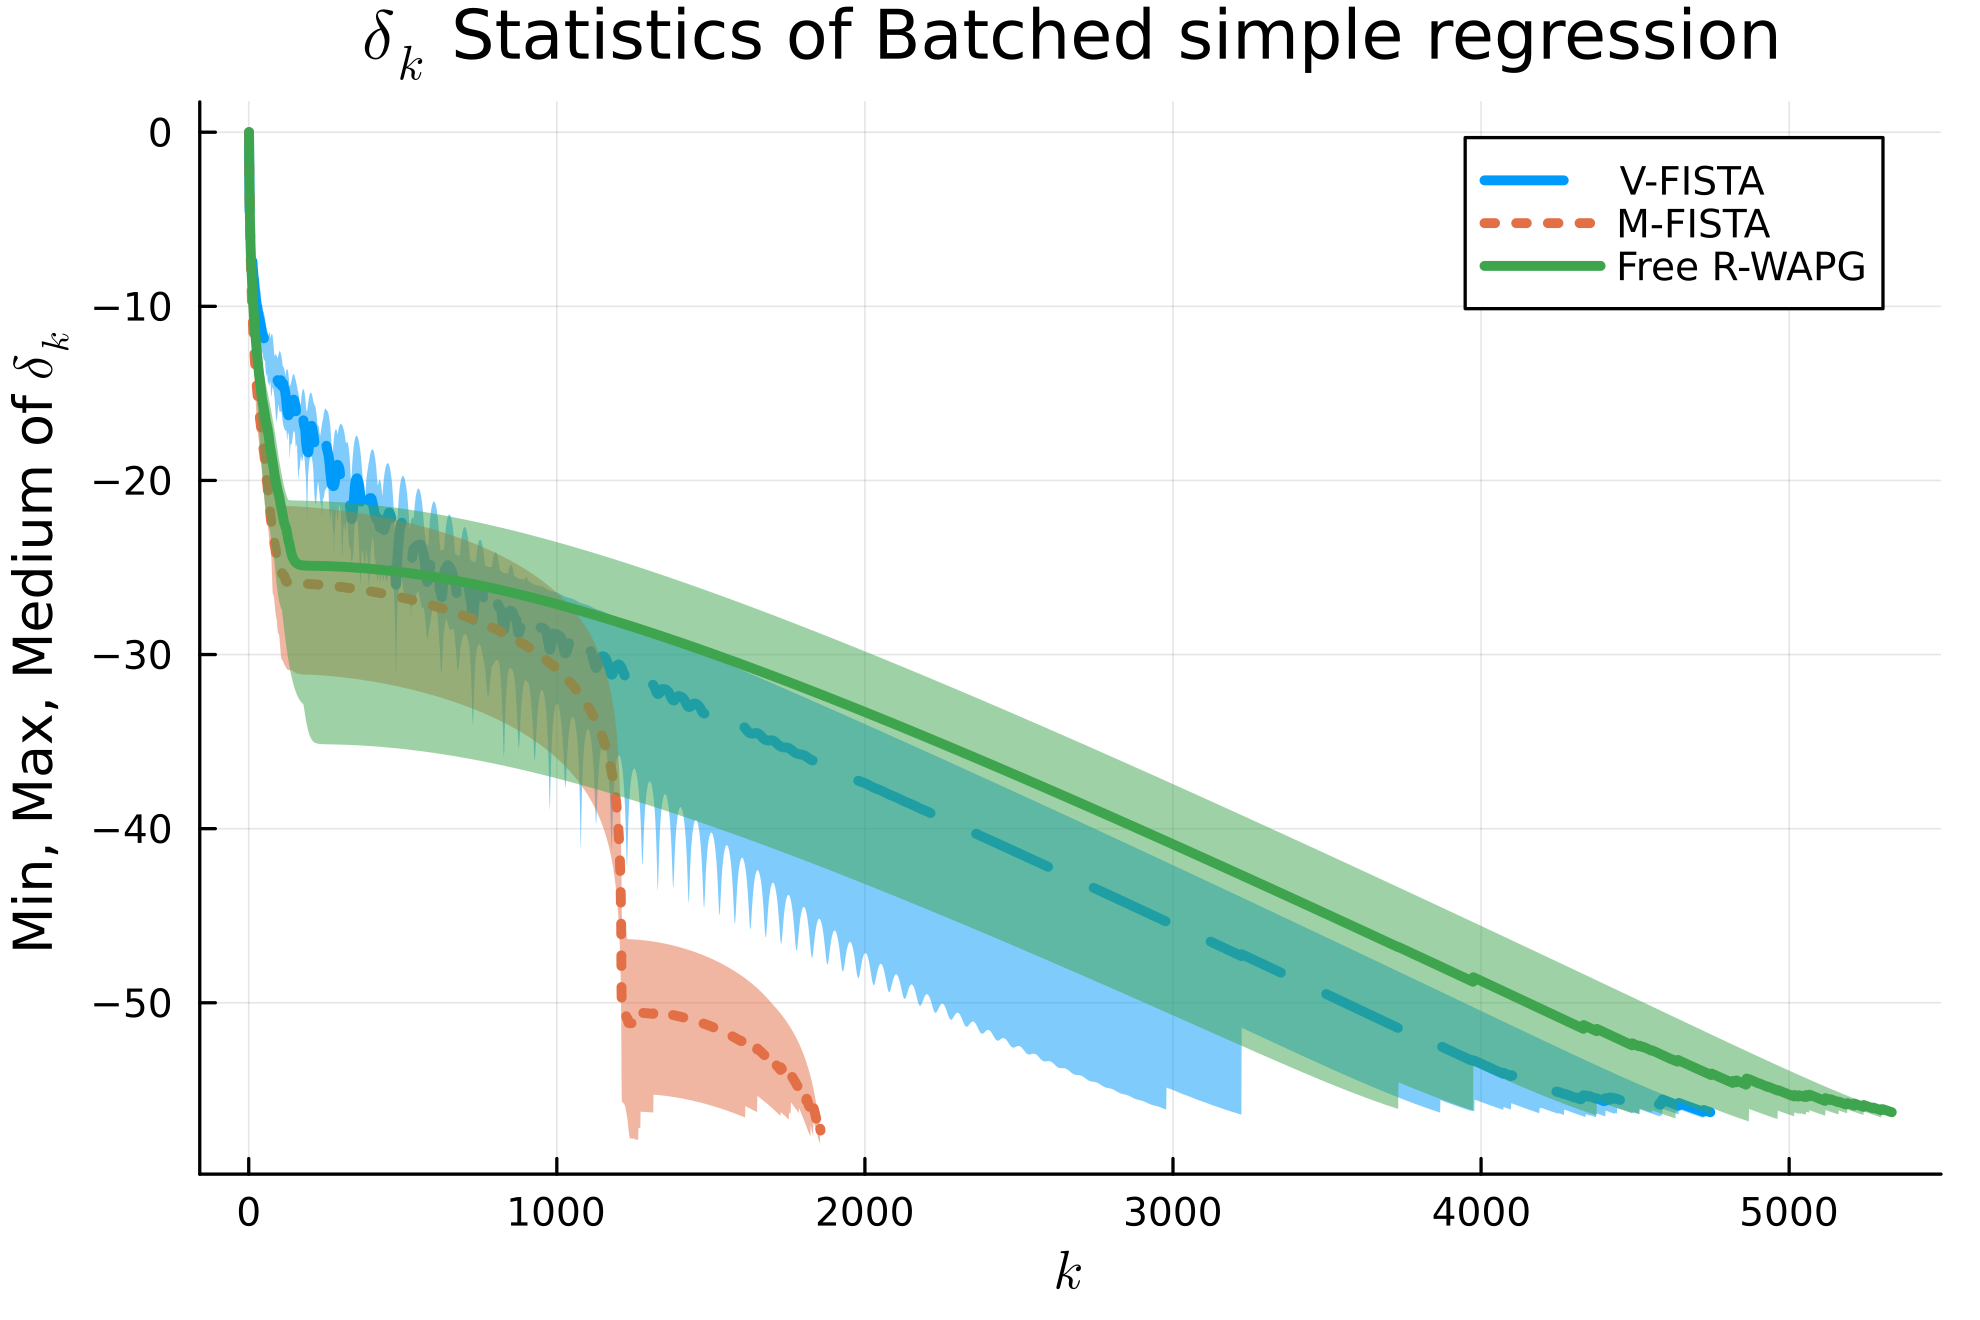
\includegraphics[width=\textwidth]{assets/simple_regression_batched-256.png}
                \caption{$N = 256$, simple convex quadratic.}
            \end{subfigure}
            \hfill
            \begin{subfigure}[b]{0.47\textwidth}
                \centering
                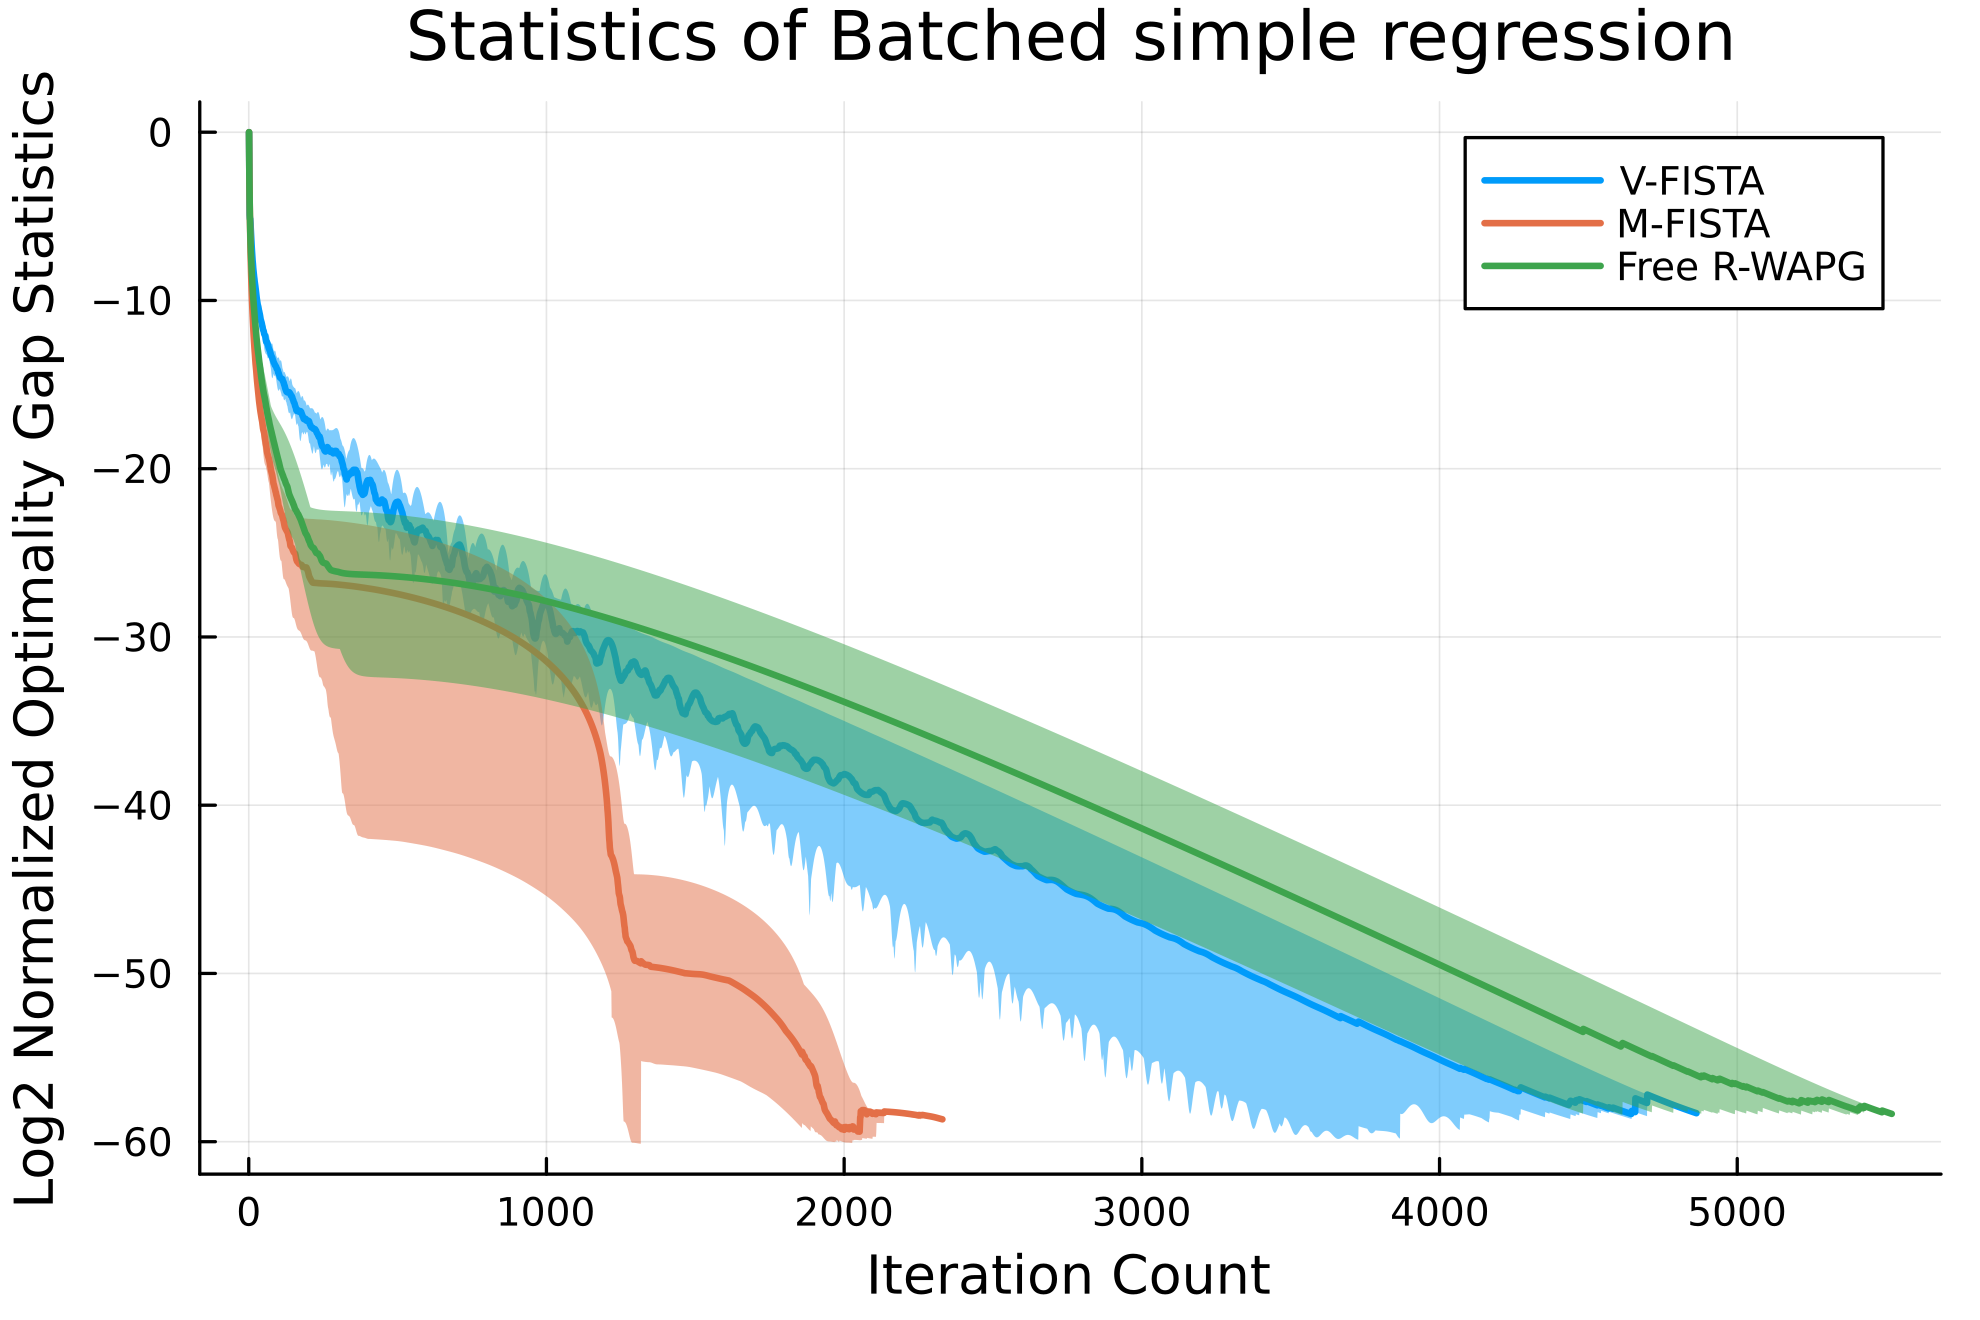
\includegraphics[width=\textwidth]{assets/simple_regression_batched-1024.png}
                \caption{$N = 1024$, simple convex quadratic. }
            \end{subfigure}
            \caption{Simple convex quadratic experiments results for V-FISTA, M-FISTA, and R-WAPG. }
            \label{fig:simple-quadratic-NOG}
        \end{figure}
        \par
        Another quantity that maybe interesting other than $\delta_k$ would be the estimated value of $\mu$ during at each iteration $k$. 
        This $\mu$ parameter should converge to the true value. 
        One individual experiment is carried out for the R-WAPG algorithm and the value of $\mu$ at each iteration is being recorded as well. 
        Figure \ref{fig:simple-quadratic-r-wapg-mu-estimates} showcases the results. 
        The values oscillate and converges to the true $\mu$ value. 
        Observe that the iteration when the estimates are nearing the true value corresponds to the iteration when the algorithm plateau away from its initial fast descent. 
        \begin{figure}[H]
            \centering
            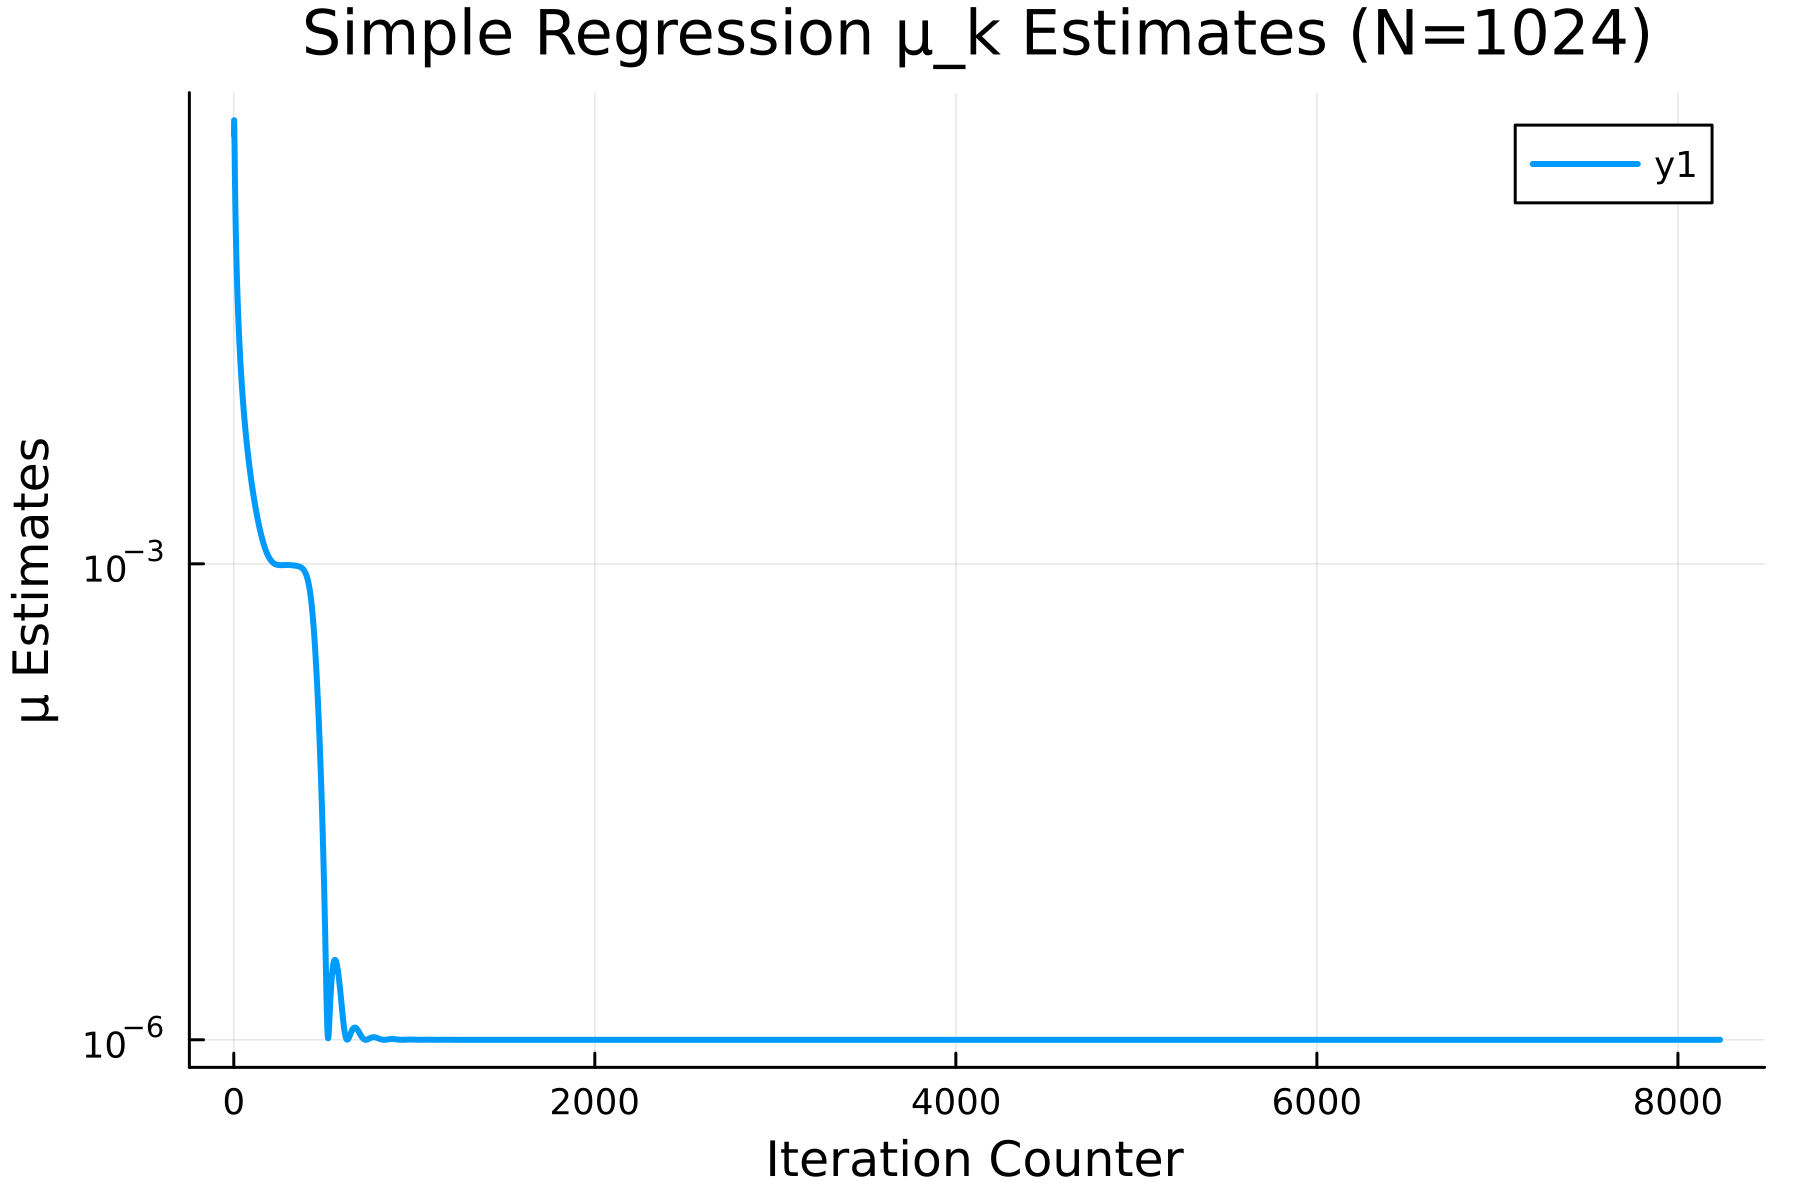
\includegraphics[width=0.64\textwidth]{assets/simple_regression_loss_sc_estimates_1024.png}
            \caption{$N = 1024$, the $\mu$ estimates produced by Algorithm \ref{alg:free-rwapg} (R-WAPG) is recorded. }
            \label{fig:simple-quadratic-r-wapg-mu-estimates}
        \end{figure}

    \subsubsection{LASSO}
        This section present results of numerical experiment for solving the (least absolute shrinkage and
        selection operator) LASSO problem proposed by 
        \todo{
            $\blacksquare$ Add reference ``Regression shrinkage and selection via the Lasso''
            \\ $\blacksquare$ Cite it. 
        }{\hl{Tibshirani}} \cite{tibshirani_regression_1996}. 
        The problem of LASSO has smooth, nonsmooth additive and the problem is given by: 
        \begin{align*}
            \min_x
            \left\lbrace
                \frac{1}{2}\Vert Ax - b\Vert^2 + \lambda\Vert x\Vert_1
            \right\rbrace. 
        \end{align*}
        The smooth part is $f =\frac{1}{2}\Vert Ax - b\Vert^2$ and the nonsmooth is $g = \lambda\Vert x\Vert_1$. 
        The objective function is coercive and the exact minimum, or minimizers are unknown. 
        We perform numerical experiments using V-FISTA, M-FISTA and R-WAPG on this problem. 
        The parameters for setting up the problem now follow. 
        \begin{enumerate}
            \item $M, N$ are constants. 
            \item $A \in \RR^{M\times N}$ is a matrix of i.i.d random variable, taken from a standard normal distribution. 
            \item $L, \mu$, the Lipschitz constant and the strong convexity constant for the smooth part of the objective are not known prior, and it's estimated through $A$ by $\mu = 1/\Vert (A^TA)^{-1}\Vert$ and $L = \Vert A^TA\Vert^2$. 
            \item $x^+ = [1\; -1\; 1 \; \cdots ]^T \in \RR^N$, it's a vector with alternating $1, -1$ in it. 
            \item Given $x^+$, it has $b = Ax^+ \in \RR^M$. 
            \item Given $A$, estimations for $L,\mu$ are given by $L = \Vert A^TA\Vert$, $\mu = \Vert (A^TA)^{-1}\Vert^{-1}$. 
            \item $x_0\in \RR^N$ is the initial guess. Its elements are random i.i.d variable realized from the standard normal distribution. 
            \item $\epsilon > 0$ is the tolerance the controls the termination criteria for test algorithms. 
        \end{enumerate}
        Experiments were conducted using V-FISTA, M-FISTA and R-WAPG with $(M, N) = (64, 256)$ and $(M, N) = (64, 128)$. 
        Matrix $A$ is fixed and the for all test algorithms and all repetitions. 
        The same experiment are repeated 30 times, but each time, we fix a different random initial condition $x_k$ for all test algorithms. 
        The aggregate statistics of $\delta_k$ are collected for all repetitions, and then grouped by the respective algorithm. 
        The results are showcased in Figure \ref{fig:batched-lasso}. 
        The bump on the curve is due to a subset of test instances of the 30 repetition where the algorithms take larger number of iterations to terminate. 
        \begin{figure}[H]
            \begin{subfigure}[b]{0.47\textwidth}
                \centering
                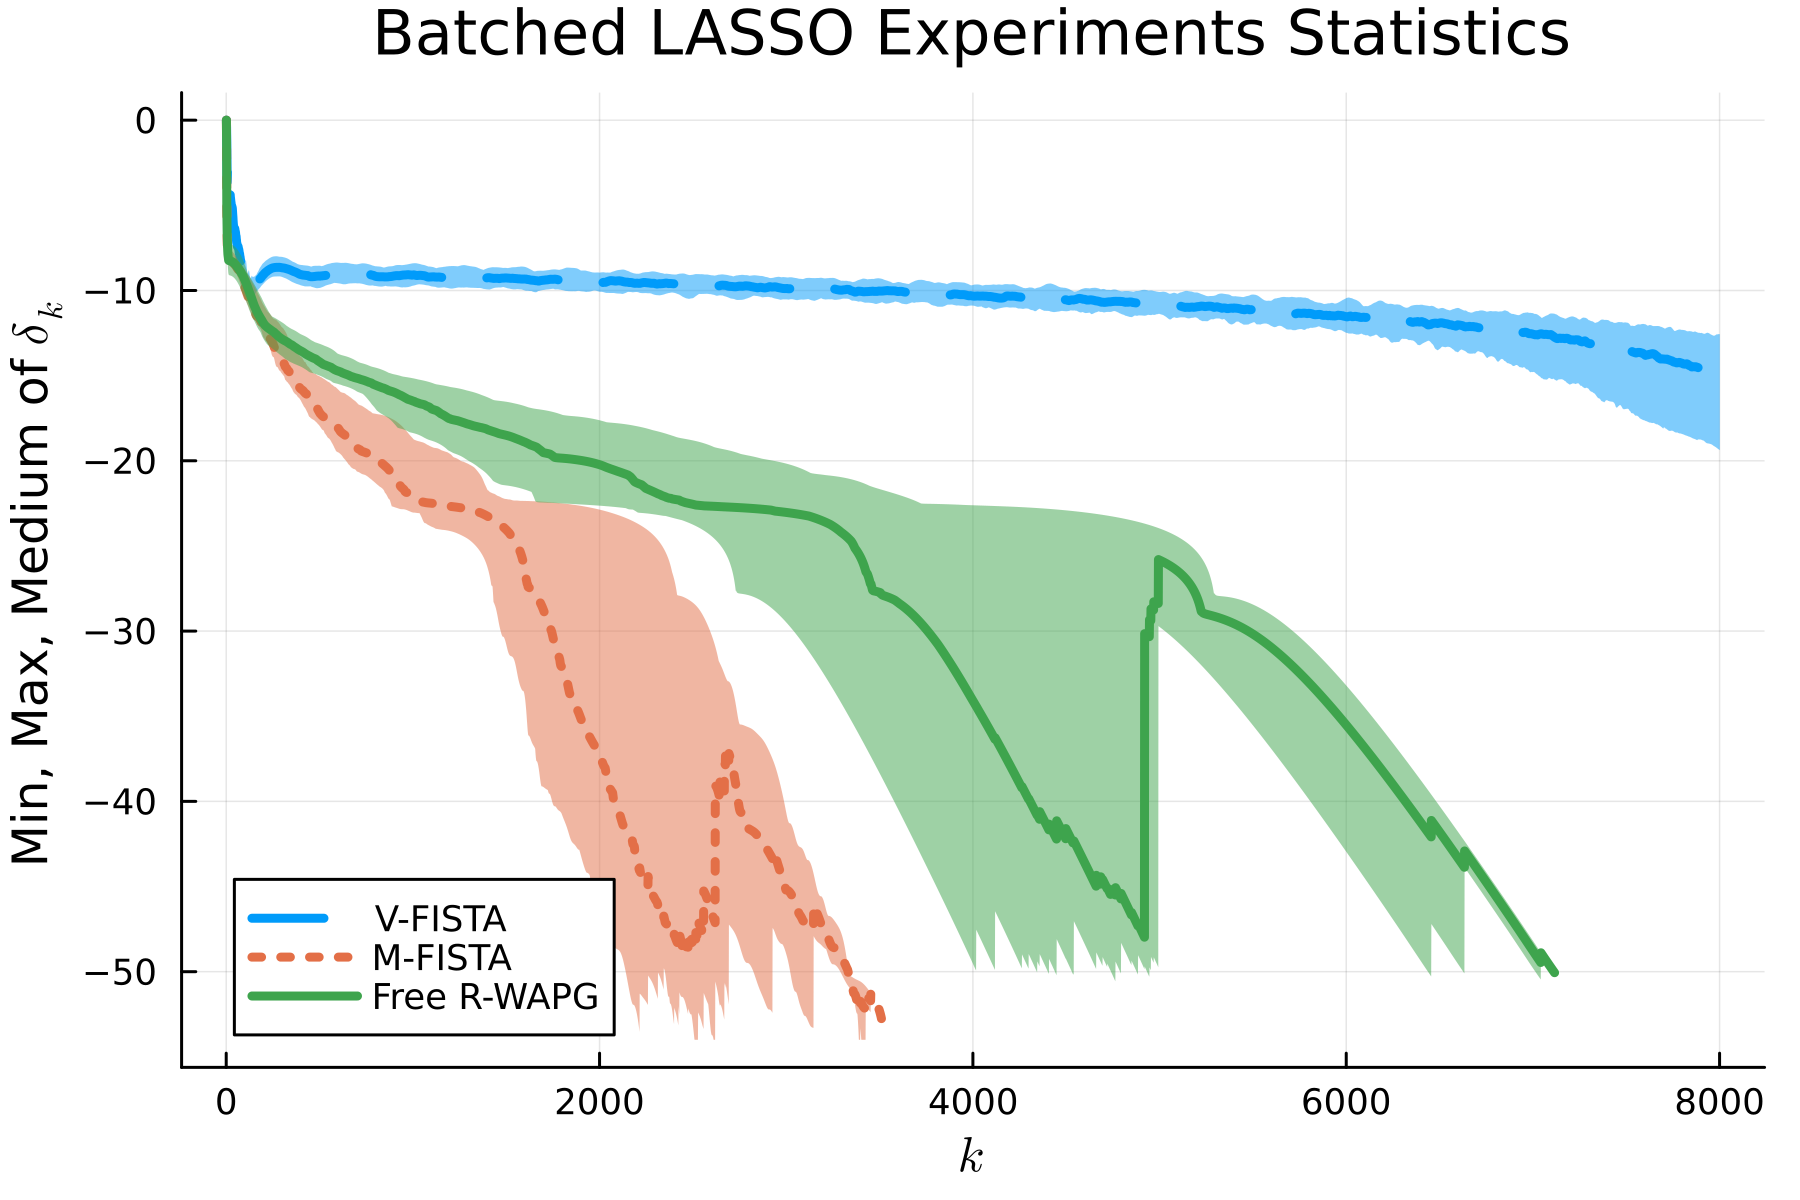
\includegraphics[width=\textwidth]{assets/lasso_batched_statistics_64-256.png}
                \caption{LASSO experiment with $M = 64, N = 256$. Plots of minimum, maximum, and median $\delta_k$ with estimated $F^*$. }
            \end{subfigure}
            \hfill
            \begin{subfigure}[b]{0.47\textwidth}
                \centering
                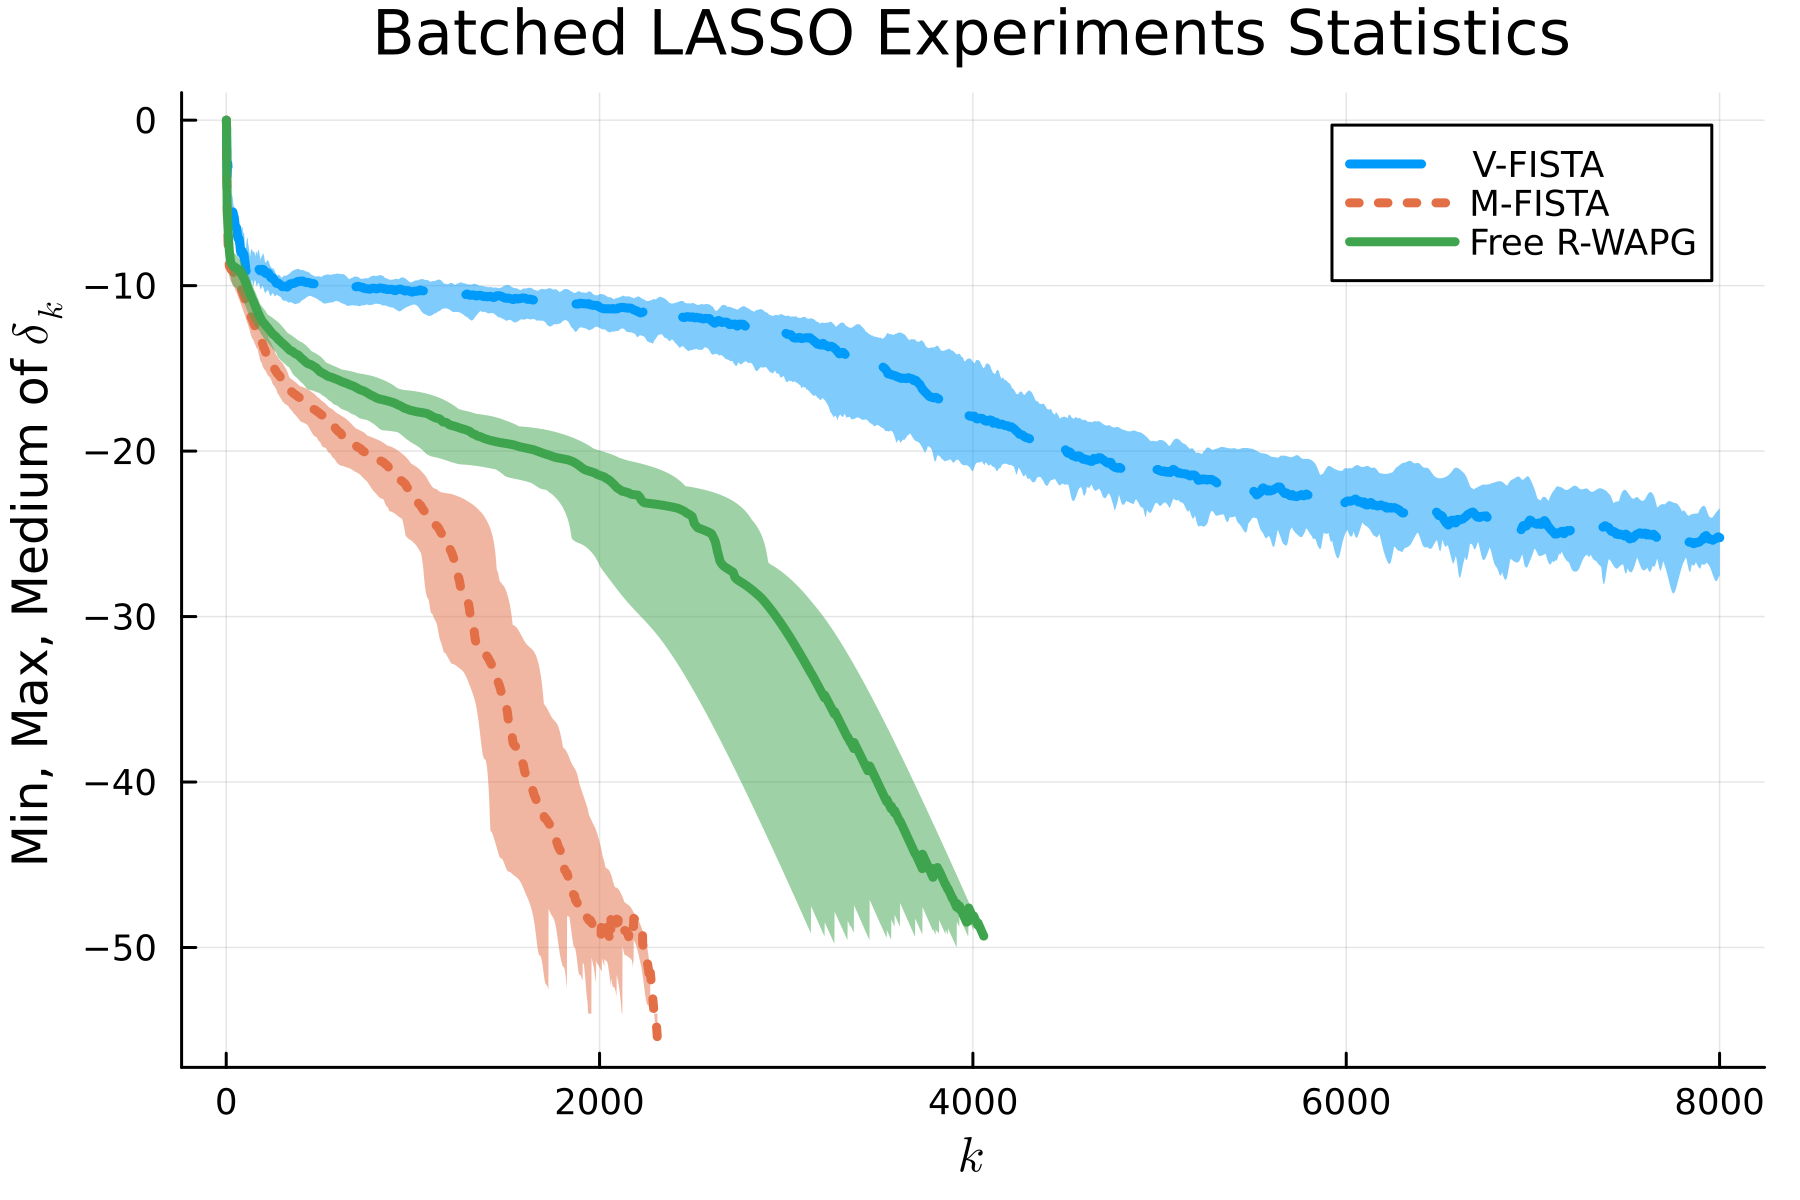
\includegraphics[width=\textwidth]{assets/lasso_batched_statistics_64-128.png}
                \caption{LASSO experiment with $M = 64, N = 128$. Plots of minimum, maximum, and median $\delta_k$ with estimated $F^*$. }
            \end{subfigure}
            \caption{LASSO experiments. }
            \label{fig:batched-lasso}
        \end{figure}
        \par
        Another quantity of interest is the estimates of $\mu$ on each iteration of the algorithm. 
        A single experiment were conducted and the estimates and $\delta_k$ are showcased in Figure \ref{fig:single-lass-mu-estimates}
        \begin{figure}[H]
            \begin{subfigure}[b]{0.47\textwidth}
                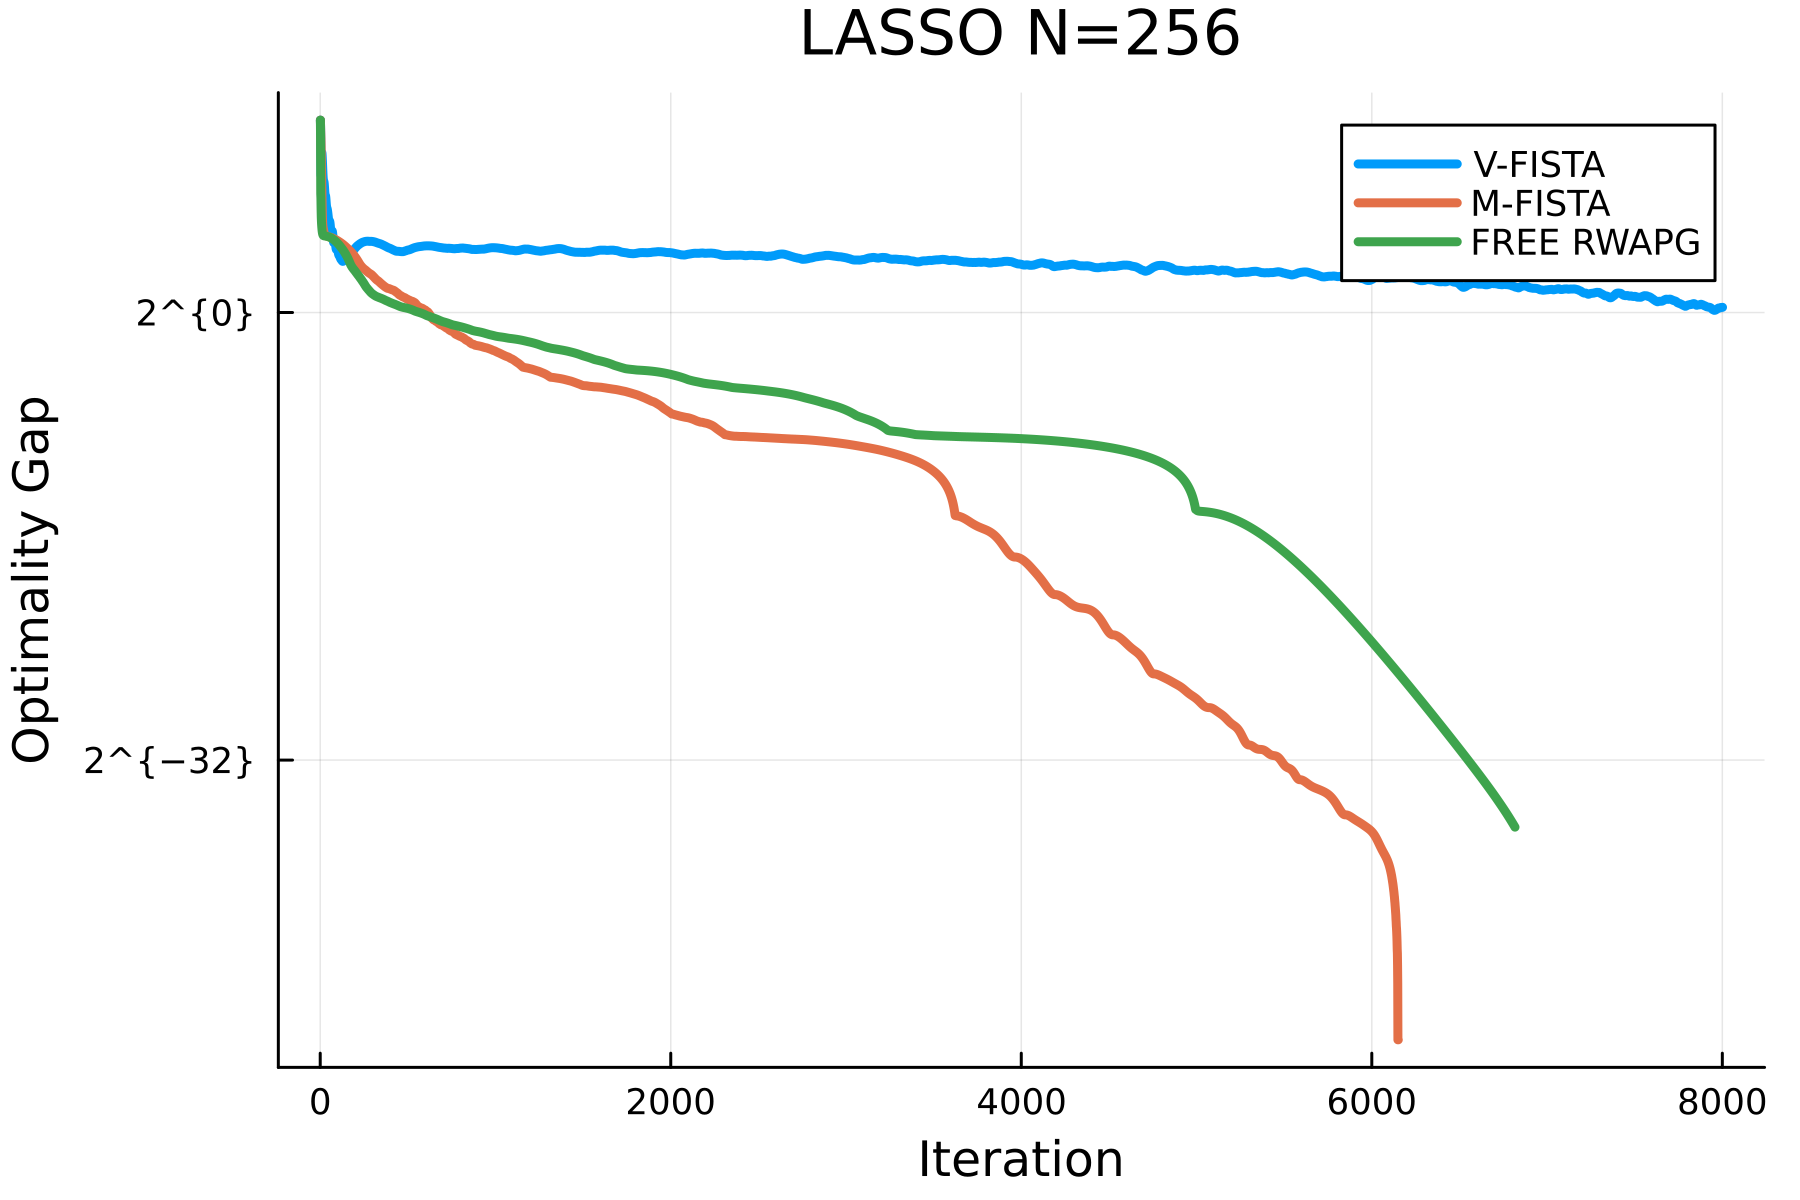
\includegraphics[width=\textwidth]{assets/lasso_loss_256.png}
                \caption{Single lasso experiment plot of $\delta_k$ with.  }
            \end{subfigure}
            \hfill
            \begin{subfigure}[b]{0.47\textwidth}
                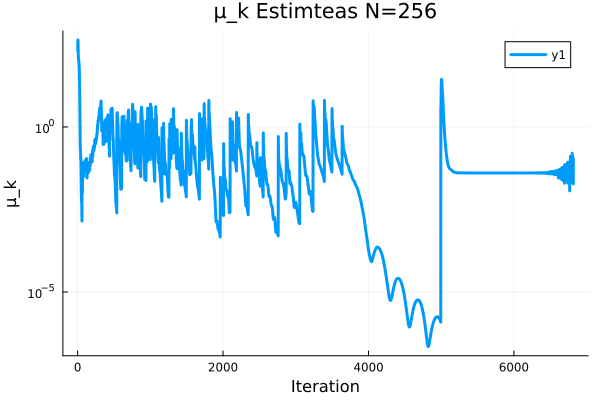
\includegraphics[width=\textwidth]{assets/lasso_sc_estimates_256.png}
                \caption{The $\mu$ estimated by test algorithms for one LASSO experiment. }
            \end{subfigure}
            \caption{A single LASSO experiment results, with $M = 64, 256$. }
            \label{fig:single-lass-mu-estimates}
        \end{figure}
        For this specific experiment showed in the figure, the estimated value of $\mu, L$ which we feed into V-FISTA are $\mu = 7.432363627613958\times 10^{-18}$ and $L = 2321.737206983643$. 
        One of the most important feature is that the estimate $\mu$ doesn't converge to the true value, but it didn't affect the convergence of $\delta_k$. 

        \subsubsection{Logistic regression}
        

\section{Catalyst accelerations and future works}\label{sec:catalyst}
    \todoinline{\noindent
        Literatures review of the topics in Catalyst acceleration method. 
        Here is a list of topics: 
        \begin{enumerate}
            \item The original accelerated PPM. 
            \item The Catalyst with weakly convex objectives. 
        \end{enumerate}
        After the literature reviews of the core literatures, move on and state new research directions and open problems. 
        There are several directions for open problem: 
        \begin{enumerate}
            \item APPM method for monotone operators instead of just subgradient, whether the same framework exists in a greater context. 
            \item Accelerated Proximal Bregman Method. 
            \item Removing smoothness assumption in Catalyst acceleration framework. 
        \end{enumerate}  
    }
    \todoinline{\noindent
        A list of relevant literatures: 
        \begin{enumerate}
            \item Güler's 1992 paper on Accelerated Proximal Point method. 
            \item Lin's, and Payquette's three trilogy paper on Catalyst acceleration for convex, non-convex Variance reduced algorithm. 
        \end{enumerate}
    }
    In this section, we assume that $F: \RR^n \rightarrow \overline \RR$ is a convex function. 
    This section reports major results from literatures concerning the method of Catalyst Acceleration. 
    \begin{assumption}
        Given any $\beta > 0$ and $y \in \RR^n$, and $F: \RR^n\rightarrow \overline \RR$ is $\mu \ge 0$ strongly convex and closed. 
        Define the model function for all $y\in \RR^n$ to be 
        \begin{align*}
            \mathcal M^{\beta^{-1}}(\cdot; y) &:= 
            F(x) + \frac{\beta}{2}\Vert x - y\Vert^2.
        \end{align*}
        We define the Moreau Envelope at $y \in \RR^n$ to be $\mathcal M^*_{\beta^{-1}}(y) = \min_{x\in \RR^n} \mathcal M^{\beta^{-1}}(x; y)$. 
        We denote $\mathcal J_{\beta^{-1}}$ to be the resolvent operator for subgradient of $F$, and $\mathcal J_{\beta^{-1}}^\epsilon$ for any $\epsilon \ge 0$ to be the inexact resolvent operator. 
        \begin{align*}
            \mathcal J_{\beta^{-1}}^\epsilon y &:= 
            \left\lbrace
                x \in \RR \left | 
                    \mathcal M^{\beta^{-1}}(x; y) - 
                    \mathcal M_{\beta^{-1}}^*(y) \le \epsilon
                \right.
            \right\rbrace. 
        \end{align*}
        Setting $\epsilon = 0$, we have the exact definition of the exact resolvent given as $\mathcal J_{\beta^{-1}}y = \mathcal J^0_{\beta}y$. 
    \end{assumption}

    Inspired by accelerated proximal point method from Güler \cite{guler_new_1992}, and inexact proximal point method of Rockafellar 1976 \cite{rockafellar_monotone_1976}, Lin \cite{lin_universal_2015} proposed a generic method taking inspirations from the convergence claims of Accelerated proximal point method to accelerated the convergence rate of first order variance reduced incremental method. 
    The class of variance reduced method is vast, but to use the most relevant feature of this class of first order method is that they are stochastic method that is not slower than full gradient descent in complexity. 
    \todo{
        $\blacksquare$ Add the bib for Mark Schmidt introductory paper RV methods.  
        \\ $\square$ Cite it. 
    }{\hl{See Gower's guide}} for more information on variance reduced methods in machine learning. 
    In brief, a variance reduce method (VRM) is a type of stochastic gradient methods that stablizes the current estimate using information of the gradient at previous iterates. 
    In each iteration, only the gradient of a few samples are accessed but attain overall better complexity because the variance of the estimated gradients are reduced. 
    \todoinline{
        We can then list some citations and references to commonly known variance reduced method here. 
    }
    \par
    The parts coming will introduce the algorithms, explain key innovations behind the algorithm, and key variants of the algorithm. 
    The section at the end will give future works and extensions of the Catalyst framework. 

    \begin{definition}[Lin's Universal Catalyst Acceleration]\label{def:lin-catalyst}\; \\
        Let the initial estimate be $x_0 \in \RR^n$, fix parameters $\kappa > 0$ and $\alpha_0 \in (0, 1]$. 
        Let $(\epsilon_k)_{k \ge 0}$ be an error sequence chosen for the evaluation for inexact proximal point method. 
        Initialize $x_0 = y_0$. Then the algorithm generates $(x_k, y_k)_{k\ge 0}$ for all $k \ge 1$ such that: 
        \begin{align*}
            & \text{find } x_k \in \mathcal J_{\kappa^{-1}}^{\epsilon_k} y_{k - 1}, 
            \\
            & \text{find } \alpha_k \in (0, 1) \text{ such that } \alpha_k^2 = (1 - \alpha_k)\alpha_{k - 1}^2 + (\mu/(\mu + \kappa))\alpha_k,
            \\
            & 
            y_{k} = x_k + \frac{\alpha_{k - 1}(1 - \alpha_{k - 1})}{\alpha_{k - 1}^2 + \alpha_k}(x_k - x_{k - 1}). 
        \end{align*}
    \end{definition}
    \begin{remark}
        The above algorithm is Algorithm 1 from Lin's first paper on Catalyst Acceleration \cite{lin_universal_2015}. 
        The explicit formula for $\alpha_k$ is the larger root of solving the quadratic equation given by: 
        \begin{align*}
            \alpha_k &= 
            \frac{1}{2}\left(
                - \alpha_{k - 1}^2 - q + \sqrt{(q + \alpha_{k - 1})^2 + 4 \alpha_{k - 1}}
            \right), 
        \end{align*}
        where $q = \mu/(k + \mu)$. 
        Lin suggests different choices for the parameter $\kappa > 0$ depending on the algorithm chosen to evaluate the subroutine for $\mathcal J_{\kappa^{-1}}^{\epsilon_k}y_{k - 1}$. 
        The choice of $\epsilon_k$ depends on the estimated optimality gap $F(x_0) - F^*$ where $F^*$ is the minimum of $F$ and whether $\mu > 0$ or $\mu = 0$. 
    \end{remark}
    Much of the heavy lifting of constructing the algorithms were done through the method of estimating sequence introduced back in Definition \ref{def:nes-est-seq}. 
    The convergence of the algorithm made use of an inexact version of the proximal gradient inequality (similar to Theorem \ref{thm:prox-grad-ineq}) stated as Lemma A.7 in \cite{lin_universal_2015}. 
    This lemma is instrumental for deriving an inexact variant of the estimating sequence $\phi_k^* \ge F(x_k) + \xi_k$. 
    The sequence $\epsilon_k$ is compacted and bounded under an upper bound parameterized via the sequence $(\epsilon_k)_{k \ge 0}$. 
    The convergence proof from Lin was inspired by 
    \todo{\noindent
        $\blacksquare$ Add bib, the paper is 
        \\
        $\square$ Cite. 
    }{\hl{Schmidt's Inexact Proximal Gradient method. }} 
    \par
    The technique of Estimating sequence results in depressingly long proof making it unsuitable for exposition here, however every significant piece of innovation is covered in details in our most recent Fall Winter 2024 MATH 590 report. 
    \par 
    The following parts will complement the report and describe ideas on Lin's idea for choosing, termination criteria of the inner loop to evaluate $\mathcal J_k^{\epsilon_k} y_k$ in his second paper on Catalyst Acceleration \cite{lin_catalyst_2018}. 
    To elucidate the matters consider the model function $\mathcal M^{\kappa^{-1}}(x; y)$ is $\mu + \kappa$ strongly convex, and therefore it admits the Polyak error bound condition: 
    \begin{align*}
        (\forall x\in \RR^n) \quad 
        \mathcal M^{\kappa^{-1}}(x; y) -
        \mathcal M_{\kappa^{-1}}^*(y) 
        &\le (1 + \mu)\dist
            \left(\mathbf 0, \partial \mathcal M^{\kappa^{-1}}(x; y)
            \right). 
    \end{align*}
    By choosing $x$ such that $\dist(\mathbf 0, \partial \mathcal M^{\kappa^{-1}}(x; y)) \le \epsilon$, it ensures $x \in \mathcal J^\epsilon_{\kappa^{-1}}(y)$. 
    Unfortunately in practice, this is not used because a full gradient evaluation on the model function $\mathcal M^{\kappa}(\cdot; y)$ is costly (compare to the small amount required for variance reduced incremental method), so Lin suggested alternatives of Inner Loop Termination Criteria to make Catalyst acceleration competitive in practice. 
    \todoinline{
        Elucidate things by considering: 
        \begin{enumerate}
            \item What is the suggested error sequence $\epsilon_k$ for different type of objective function? 
            \item What are some conditions for achieving inexact evaluation up to the given accuracy $\epsilon_k$? 
            \item What are the convergence claims for these different types of termination criteria. 
        \end{enumerate}
    }
    \subsection{Error sequence and convergence claims}
    \subsection{Inner loop termination criteria}    
    \subsection{Potential future research}

    

\section{Methods of inexact proximal point}\label{sec:inexact-prox}
    

\section{Nestrov's acceleration in the non-convex case}\label{sec:nes-acc-ncnvx}
    


\section{Using PostGreSQL and big data analytic method for species classification on Sentinel-2 Satellite remote sensing imagery}


\bibliographystyle{siam}
\bibliography{references/proposal.bib}
\newpage

\appendix

\end{document}
